%
%  lars must fix dexcription of ttplot, look for lars
%  peter, put in new figure 15, is made
%  jan 24 2012 jh: many smaller changes
%  may2  2012  jh: document test 107 for xnear etc
%
%\chapter{USING SEISAN}
\chapter{Using SEISAN}
\label{chap:using-seisan}

Once the system has been installed, it is ready to use.  Usually all work should be done in the WOR directory or on a multi user system from your own directory. To move to WOR, type WO. Unless you have to do system work, it will not be necessary to move to any other directories.  However to do so, just type the first two letters of the directory name like DA to move to the DAT directory. On a PC the Edit editor is default (invoked with command edit), and on SUN the vi editor. 

The system has two basic \index{Modes of operation}modes of operation. The first is to work interactively with the database. That means jumping around from event to event, plotting, interactive phase picking, locating, deleting, typing, editing or appending events (S-files). This mode is invoked with the command \index{EEV}EEV, which uses several programs, controlled by a driver program and is intended for testing and editing of single events. Once the input data seems OK, the second mode of operation can be used. 

On Windows95/98/2000/NT, program SEISAN is equivalent to EEV and 
whenever EEV is mentioned, this is meant to also include W95/98/NT, 
SEISAN, see section \ref{subs:eev-win}.\index{Windows95} 

The second mode is more like traditional data analysis where single programs are made to work on the whole or part of the database. In this mode the updated \index{S-file}S-files and \index{CAT-file}CAT-files are created. Examples are also plotting of epicenters, waveform data or searching for data fulfilling certain criteria. 

The system comes with a test data set from different networks, mainly the Norwegian National Network for the time periods 199309 to 200002. The data has waveform data in different formats. The data set includes events from both local and teleseismic distances. The installation of test data is separate from installation of SEISAN.  

If you want to try the system, go directly to section \ref{sect:interactive} 
to get a feeling for how the system works.   

SEISAN problems: Some of the most common problems have been 
collected in the index under the header "Problem". 

%\textcolor{red}{lo-change:}
\section{SEISAN TRAINING COURSE} 
%\label{chap:training}

The document `Computer exercises in processing earthquake data using 
SEISAN and introduction to SEISAN' which is a tutorial for new users 
as well as experienced users, is included in the distribution. The 
testdata used in the exercises need to be installed, see %section 3
chapter \ref{chap:installation}. 
Going through the exercises of the tutorial might be the best way 
to learn SEISAN. The document is given as PDF file 
(\texttt{seitrain.pdf}) in the INF directory. 

The main goal of the introductory training course is to become familiar 
with the database program EEV, the plotting program MULPLT and the 
location program HYP. Of course additional reading of relevant sections 
in this manual is required. The basic exercises can be completed within 
one or two days, while the advanced exercises take more time. 

%Content of the exercises 
%
%\begin{enumerate}
%\item[1] SEISAN basic exercises 
%\item[2] Phase reading 
%\item[3] Response files and seismic formats 
%\item[4] Signal processing 
%\item[5] Earthquake location 
%\item[6] Magnitude 
%\item[7] Focal mechanism 
%\item[8] Spectral analysis and Q 
%\item[9] Operation and earthquake statistics 
%\item[10] Array analysis 
%\item[11] Analysis of a data set 
%\item[12] Data manipulation and import and export of data 
%\end{enumerate}

\section{Short user guide}
\index{Short user guide}\index{Common tasks in SEISAN} 

The SEISAN manual has been divided into sections describing the individual programs. However, many tasks require the use of many programs and it is not always easy to find what can be done and which programs to use. The following section intends to give an overview of some general problems that SEISAN can work with and a list of programs to use. The following tasks have been identified: 

\begin{itemize}
\item[-]Routine processing: Phase picking, hypocenter location and magnitudes 
\item[-]Determination of source parameters: Fault plane solution, stress drop, etc 
\item[-]Determination of back azimuth and apprent velocity using arrays and networks 
\item[-]Crustal structure: Velocities, layer thickness and attenuation 
\item[-]Seismic catalogs: ISC data, database management, completeness, statistics, etc  
\item[-]Seismic hazard: Attenuation, catalogs, and soil response 
\end{itemize}

\textbf{Routine processing}

The main work of a seismic observatory is to quickly process and organize incoming data from different sources. SEISAN has a simple time ordered database (see later section) and a set of programs for these tasks. The most important programs are: 

EEV: The EEV program is the interactive program for working with single events in the database. The program is used to navigate in the database to find a given event as well as for housekeeping (splitting, merging and deleting events). Once an event has been selected, a large number of options are available like phase picking, earthquake location, fault plane solution, macroseismic information etc. All results of the interactive processing are stored in the database (S-files).  

MULPLT: \index{Trace plotting}\index{Phase picking}This is the general plotting and signal analysis program and can be used to pick phases and amplitudes, correct for instrument response, produce Wood-Anderson seismograms for determining Ml, simulate WWSSN SP and LP records, determine azimuth of arrival for 3 component stations, rotate seismograms, display theoretical arrival times for IASP91 phases to help identifying global phases and do spectral analysis. MULPLT can be used from EEV or as a stand-alone program. 

FK and PFIT Determining apparent velocity and back azimuth using an array of a local /regional network. 

HYP: This is the general program for hypocenter location and is based on HYPOCENTER \citep{lienert1986,lienert1995}. The program can use nearly all common crustal and global phases (8 character ISC codes), locate teleseismic events using the IASP91 model and use observed azimuth and apparent velocity. The program can therefore be used with all types of input data whether from single stations or arrays. HYP can be used from EEV or as a stand-alone program. Apparent velocity is currently only used for starting location. 

EPIMAP: This is the general hypocenter plotting program for making epicenter maps and hypocenter profiles. The hypocenters can be plotted with elliptical error ellipses and EPIMAP can also be used for interactive selection of events in polygon areas.  For plotting hypocenters, there is also an interface to GMT.  

BUL: The function of this program is to produce a bulletin. The user can tailor the appearance to local needs and the program can produce bulletins of hypocenters only or both hypocenters and phase readings. 

In addition to the above programs, several programs are available for database creation, input and output of large data sets and conversion and manipulation of waveform data.  

In order to get an idea of how routine processing works, some examples of routine processing will be given below. 

\textbf{Case A:} Telemetry network with 32 channel central recording

The network generates waveform event files, which are transferred to SEISAN. The tasks are: 

\begin{enumerate}
\item[1:]
Convert waveform files to SEISAN format or any of the other formats used by SEISAN. It is likely that the format is MiniSEED in which case no conversion is needed. (many events can be converted in one operation). Inspect events with MULPLT. From MULPLT, false triggers are deleted and real events are put into the database. Events are at this stage identified as local, regional or distant. Phase picks can be done at this stage, but is usually done later. 
\item[2:]
Interactive phase picking, earthquake location, magnitude etc done with EEV.  Automatic phase picking is also possible at this stage. 
\item[3:]
Database is updated (UPDATE) once a suitable interval has been processed interactively, usually a month. Updating means permanently storing the hypocenters etc in the database. 
\item[4:]
Make hypocenter maps with EPIMAP. 
\item[5:]
Produce a bulletin with BUL. 
\end{enumerate}

\textbf{Case B:} 3 telemetry networks and one broad band station

The routine is the same as above except for one additional step between 1 and 2. Since several data sets are available, some of the detections from different networks or the broad band station might correspond to the same event. There are now two options. The first is to merge the waveform files for corresponding events and then put the events into the database. The second option is to put all real events into the database and then do the merging from EEV. 

\textbf{Case C:} A mix of stations and networks and additional phase readings

The steps are as in case B except that before step 2, the additional phase data is put into the database. In this case the merging of events must be done with EEV 

\textbf{Case D:} A network recording all data in continuous mode into a SEISAN continuous data base. In addition, there is likely to be network wide triggering put into SEISAN. In this case it is a question of inspecting the triggers with EEV/MULPLT as above and possibly extract additional data out of the continuous data base and put it into the event data base. 

It should be noted that data collection and step 1 to 3 is fully automated using SEISNET \citep{ottemoller1999}\index{SEISNET}. 

Example of using EEV for interactive processing: 

Find event in default database nearest the given date and time: EEV 1999020303\newline 
Once EEV is started, an EEV prompt is given and different EEV options 
are available. Examples are:
E: Edit event, P: Plot event, L: Locate event, F: Make fault plane solution, d2201: Find event nearest day 22 at 01 hour, MAP: Start EPIMAP to show earthquake location and SAC: Start SAC processing of event using all parameter and waveform data from SEISAN database. 

The above examples have mostly described the interactive processing of single events. However, once the data is in the database, operations can be done on the whole database, for any time interval or for events fulfilling certain criteria (like magnitude, area etc). Examples are relocating events, extracting data and determining coda Q. 

\textbf{Source parameters}

The routine processing normally produces magnitudes and hypocenters. The fault plane solution can be determined using polarities and one event (Snoke et. al., 1984). Composite fault plane solutions can also be made. A second way of determining fault plane solution is to synthetically model the waveforms using the modeling programs. In addition, seismic moment, stress drop and seismic source radius can be determined by doing spectral analysis or spectral modeling. This can also be done automatically with AUTOSIG. The moment tensor of local earthquakes can be determined by inverting the amplitudes of the Pg and Sg waves \citep{ebel1990}\index{BOUSEI} 

The full wave modeling programs integrated with SEISAN, are written by \citet{bouchon1981} and \index{Herrmann}Herrmann (Herrmann,1996). The ray-tracing program is based on WKBJ and written by \citet{chapman1988} and integrated with SEISAN by Valerie Maupin. All the above programs are executed from EEV in order to use known source parameters. 

\textbf{Crustal structure and Q}

A large database can be a good source of information for determining structural parameters and SEISAN provides several programs to determine the crustal structure and Q. Using seismic arrival times, it is possible to invert for the crustal structure using the VELEST program \citep{kissling1994}. It is also possible to do forward modeling using the location program for a large number earthquakes, since it at the end of a run, a summary of average station travel time residuals and event RMS is given. A special option of HYP is to locate a data set with all permutation of a given range of models in order to find the model giving the lowest RMS. 

Deep earthquakes under a local network produce clear phase conversion at crustal interfaces \citep{chiu1986}. They can be modeled with one of the full wave modeling programs both with respect to amplitude and arrival time. 

SEISAN can, when displaying surface waves, make spectral files ready to be processed for surface wave dispersion with Herrmann's programs (Herrmann, 1996). 

Attenuation can be determined using the coda Q method for local earthquakes (CODAQ). \index{CODAQ}The coda Q program will calculate q for a series of events and stations at given frequencies. Average values are calculated and a q vs f curve is fitted to the calculated values. The principle for calculation is the standard coda q method, whereby a coda window is bandpass filtered, an envelope fitted and the coda q at the corresponding frequency calculated \citep{havskov1989}. The SPEC program will determine Q by calculating spectral ratios or the near surface attenuation using the spectral decay method. An alternative is to use spectral modeling where Q, stress drop and seismic moment are modeled simultaneously. 

\textbf{Catalog and database work}

\index{Catalog work} Once a large database has been created, several programs are used to manipulate and analyze the data. The catalog can be searched for a large number of parameters. Selection criteria are: Magnitude range, magnitude types, event types (e.g. local, distant, volcanic, explosion), latitude, longitude and depth range, RMS of travel time residuals, number of stations used in the location, felt events, number of polarities, presence of certain stations etc. Events can also be selected in an area with the program used for hypocentral plots. \newline
A very useful source of data is the ISC. Data from ISC CD ROM's can be read and converted to SEISAN format (hypocenters and phase data) and put into a database. The data can then be used for 
e.g. seismic hazard, fault plane solution or it can be relocated. A general task with catalogs is to homogenize magnitudes. Magnitude relations between e.g. Mb and Ms or Ms from one agency to Ms from another agency can be done with the program MAG. The program will also convert one magnitude to another once the linear regression has been determined. Event statistics can be made with STATIS and b-values calculated with BVALUE. The number of events as a function of time is plotted with CATSTAT. 

\textbf{Seismic hazard}

Probabilistic earthquake hazard computations is done, using the EQRISK program \citep{mcguire1976} or the CRISIS99 program \citep{ordaz1991,ordaz1999}. EQRISK computes seismic hazard in terms of probabilities of exceedence vs earthquake intensity measures such as peak ground acceleration (PGA), for a given site or a grid of sites for up to eight different return periods.  The site amplification is calculated with the SPEC program. This is used for making spectra of many seismic signals in a semiautomatic manner. The program is intended for two purposes: (1) making relative spectra for a series of pairs of stations terminated by the average spectra, (2) Making a series of spectra for a number of stations and events. The spectra can be corrected for distance, q, and instrument response. \newline
This section involves a large number of programs and a more detailed 
description is given in section \ref{sect:risk-prog}. 

\section{Getting data into the database}

The first requirement for interactive work with the event editor EEV is to get the data into the database. 

There are two ways to get data into the database, as described in 
section \ref{subs:with-digi-data} and \ref{subs:without-digi-data}. 
It is of course possible to make the individual \index{S-file}S-files 
directly in the REA directories with the editor. This would be rather 
slow, and be against the philosophy of the system. However, it is 
mentioned in order to point out how simple the database structure is. 

The SEISAN system can be used with or without digital data, the only difference to the directory structure is that the WAV and CAL directories are present when using digital waveform data.  However the way of getting data into the database differs in the two cases and will be described separately. 

\subsection{System with digital data}
\label{subs:with-digi-data}
\index{Digital data} 

This means that the original data is individual digital event waveform files generated by some data acquisition system. The waveform data can be stored in SEISAN, GSE and SAC format as single or multi trace files. The files that are used in conjunction with the database are normally stored in WAV but can also be in the user's directory, e.g. WOR.  The normal scenario would be that \index{Multiplexed files}multiplexed files would be transferred from a digital field station, demultiplexed and converted to SEISAN waveform format. Programs are provided to convert from most of the popular waveform formats like MINISEED, GSE, PCSUDS and from commercial recorders. It is most practical to initially put the files in WOR, check the events for false triggers, save the true events in WAV, make the corresponding S-file and a hardcopy of the digital data. \newline
All of this can be done with the program \index{MULPLT}MULPLT. The program plots channels from a single waveform file. The user can then interactively decide if this is an event to keep, in which case an S-file is created in the database and the event is moved to WAV. 

Alternatively, all new waveform files can be auto-registered into the database (AUTOREG) and all checking takes place from EEV. 

When digital data is the input to the analysis system, MULPLT is the 
program to use to get data into the database. From there on further 
analysis can be done with EEV (picking phases, locating and editing). 
MULPLT is also the program used with EEV. For more details on MULPLT, 
see detailed description in section \ref{sect:mulplt}. 

\subsection{System without digital data} 
\label{subs:without-digi-data}

In this case the user would get phase data from other sources, e.g. analog seismograms or files with readings from other stations and agencies. These files are assumed to be written in Nordic Format. Conversion can be done from other formats like ISC, NEIC and HYPO71. 

If a user already has a file with one or several events in Nordic Format, this file can be \index{SPLIT}split up into single files which are copied (from any directory) into the database by using the command SPLIT. Creating a new file in Nordic Format can also be done with the program \index{NEWEVE}NEWEVE (use command NEWEVE). 

The SPLIT program then reads the NEWEVE output file and writes out 
single S-files with correct names either in the current directory 
(default) or in the database specified (BER or another). The reason 
that the database specifically must be given is that the user should 
not accidentally put data into the database (see section \ref{sect:split}). 

\subsection{Database security}
\index{Duplicate ID}

\textbf{Duplicate ID:}
\index{Database security}

Since the database consists of single files with names corresponding 
to time down to the second as well as the event type (L, R or D) it will sometimes happen that two events will get the same name. Thus copying in a new event with the same name could overwrite the existing event, and the user would never know. In SEISAN, from version 5.0, some security has been put in. New data can enter the database with 4 programs: SPLIT, EEV, MULPLT and AUTOREG. With all programs, the user will be prompted if a new event is about to overwrite an existing event. Both SPLIT and EEV have the possibility to create alternative ID's if the user wants both the new and old event, while MULPLT and AUTOREG just offers the possibility to skip a double event. If a new ID is created, an attempt will be made to use a time one second later. If that also corresponds to an existing event, the next second is attempted etc. This allows for 60 events to be registered in the database with the same minute and event type. If an event has got the ID changed, the header line in the file is NOT changed, however the ID line is of course changed. This will be indicated on the ID line with a `d' at the end of the ID number. 

\textbf{Deleting events:}

\index{Delete event} Event here means S-file in the database. Events are only deleted when using EEV, either with the EEV delete command D or the EEV append command A. In both cases, the deleted event is stored in the DELET database before being deleted from whatever database. Even if the system contains many databases, there is only one DELET database. This means that deleted events from different databases are mixed in DELET. In order to restore an event, enter DELET database with EEV and copy the deleted event back with the C command. It is up to the user to manually clean up the DELET database. \newline
There is one more final security. If an event has been deleted from a database, but an UPDATE has not yet been made, the event might be in the CAT part of the database and can be extracted by SELECT or the editor. 

\subsection{Data base tools, content and checks}

Content of data bases, program BASE:

In the REA directory, a binary file called REA.LOG contains information about number of events in all data base. Initially the file has no information, but each time programs EEV, HYP, UPD, CHECK\_BASE or COLLECT are executed, the information is updated for the months accessed. The information can be displayed with program BASE, which first shows available data bases and the user, can then select one to get info for particular months. Make sure to use right case for data base names, always in upper case on Unix systems. The program is still a bit experimental !! \index{BASE}\index{REA.LOG}\index{Data base content} 

Check content of S-files for magnitudes and residuals etc, program CHECKRE:

The program can read data bases or CAT files and check events for large residuals, abnormal depths etch. The program is intended for quality control, the parameters hardwired in the program might not suit all. Check program source listing. 

\index{CHECKRE}\index{CHECK\_BASE}Check for data base related errors, program CHECK\_BASE 

The data base depends on error free S-files and that there is a correspondence between the S-file name and the event ID. This should normally be ok, however errors can occur during editing or there can be program crashed producing errors. The program reads the data base and checks for: 

Missing ID lines: If ID line is missing, it can be put in manually or doing an UPDATE. 

No correspondence between ID line and S-file name: A serious error has occurred. try to find out what is correct, the ID or the file name. An UPDATE cures the problem, however data might be lost. 

Error in S-file: All parameters are checked and files with non standard parameters are indicated. The error can be a number in a wrong position. The errors should be corrected. 

For all the above 3 cases, an index file is generated with bad S-files and  EEV can the be used directly with the index file to access the bad S-files. THIS ONLY WORKS WITH ONE DATA BASE AT A TIME. \index{Check data base}\index{Data base, check}\index{Crash, check base}

It is recommended to run check\_base in case of system crash or as a security, just before an UPDATE. 

\subsection{High accuracy in SEISAN}
\index{High accuracy} 

SEISAN can use higher accuracy than the default. The goal is to have an accuracy of 1 ms in time and 1 m in location. 

In order to write out the high accuracy numbers, a new parameter has been added to \texttt{SEISAN.DEF}. The parameter is HIGH\_ACCURACY. Setting it to 1.0 enables high accuracy operation. This parameter affects the programs MULPLT, FK, HYP and UPDATE. 

Station locations: The station file looks like before except that in order to get higher accuracy of station locations, the minutes of latitude and longitude are specified without the point. E.g. the minutes 22.122 can now be written as 22122 in the same columns as before while if the point is given, only 2 decimals can be used as 22.12. This changes do not affect any old station coordinates. Programs reading station coordinates, will use high accuracy input if available. 

EPIMAP will always read in high accuracy mode, if any high accuracy data is present, whether station locations or hypocenters. 

FK will always read high accuracy station coordinates, if available and FK can therefore now be used with very small arrays.   

Programs with output affected by high accuracy mode: 

MULPLT will write the phase readings as f6.3 instead of f5.2 like e.g. 11.234 instead of 11.23. For normal use, this is not needed and the files look better if high accuracy mode is not used. 

HYP and UPDATE writes an extra high accuracy hypocenter line which has been given type H. An 
example is  

\verbatiminput{include/high.accuracy}

\section{Interactive work with earthquake locations, EEV command}
\index{Interactive work}\index{EEV} 
\label{sect:interactive}

The idea of SEISAN for interactive work is that the user should be able to easily jump from event to event and run several different programs with one event without restarting every time. This is done with the command EEV (see below). In this interactive mode, events are picked, edited, located, moved, deleted etc. until a satisfactory solution is found. In the interactive mode, NO \index{UPDATE}UPDATING of the location in the S-file or the permanent output CAT directory is done since it is too easy in interactive mode to accidentally change something. The permanent updating of S-files and CAT directories can only be done for one or several months at a time (see UPDATE command) in order to ensure that nothing is forgotten within a month. 

Once the events have been updated, further work can be done (like searching for specific events or making a bulletin) using single programs which read directly from the database. Most of the analysis programs will also work without using the database structure that is e.g. searching in single file with many events. For more details of the analysis programs, see %section 6. 
chapter \ref{chap:prog-commands}.

\section{How EEV works}
\label{sect:eev}

It is now assumed that data has been entered into the database. The fundamental tool for the database is then the EEV program, which mostly works within the limits of one \index{Index file}month in the standard database or with whatever the user has of S-files in his own directory. Optionally, EEV can also work with several months. A special option is to use a list of files in an INDEX file, see end of this section and SELECT program. Some of the commands available within EEV are also available within programs. See below for more details on EEV. 

The EEV program reads the file names of all S-files in the database monthly directory (or local directory or index file), positions the pointer at the first event and asks for a command to be performed for the current event or to find another event. If the command is to use a program, control is handed over to that program, which on completion hands control back to EEV. In this way, many different independent programs can be used from within EEV, e.g. several different location programs can be installed.   

EEV can be started in several ways: 

EEV with one month in default database: EEV yyyymm. \newline
E.g. EEV 199201 would work on January 1992 on the standard BER database. It is here also possible to give a more precise start time like EEV 1992011520 to start with the first event at or after January 15 at 20 hrs. 

EEV with one month in alternative database: EEV yyyymm BASE.\newline
BASE is the database. To work on the NAO base, the command would be EEV 199201 NAO. 

EEV with several months in default database: EEV yyyymm YYYYMM\newline
yyyymm is start year and month and YYYYMM is end year and month. 

EEV with several months in alternative database: EEV yyyymm YYYYMM BASE\newline
yyyymm is start year and month and YYYYMM is end year and month. 

EEV to work with events is local directory: EEV\newline
Only the S-files in local directory will be used. 

EEV to work with an index file: \texttt{EEV index.out}\newline
EEV can work with an index file and the command would be \texttt{EEV index.out}, 
where \texttt{index.out} is the index file name (can have any name as long 
as it contains a `.' except when used with HYP). 
For information on index files, see \ref{sect:select}. 

Databases can have 1-5 letter names and the user specify 1-5 letters. The real names in the directory structure are always 5 letters so if the user specifies e.g. a base name of BA, the real name will be BA\_\_\_ . The full 5-letter name can also be used. 

The \index{Commands in EEV}commands in EEV mainly use only one letter unless a date or a number has to be given. To get a short explanation, type ? and you will get:   

%\verbatiminput{include/eev.help}
\verbatiminput{include/EEV.HLP}

Note: Command letters can be upper or lower case. 

Comments to commands: 

\#XXX : \index{Go to event by number or date}Go to event by number. When giving a number, only give the number of digits needed, no formatting. Thus e.g. to find event 7 or 777, write 7 or 777 respectively. If there is not an event corresponding to the parameter specified, EEV will go back to event \#1. In the number command, \# can be omitted. 

Axxx: \index{Append another event to current event}Append another event to current event. The event specified is appended to current event. All header and lines in both files are saved and put in order in the current event. The main first header is from the current event. The ID line for the appended event is saved as a comment line. The user will be questioned if the appended event is to be deleted. 

AA: Same as above using next event. 

AUTOSIG: Automatic processing with autosig program. 

B: Back one event 

BOUCH: Run Bouchon's modeling program 

BOUSEI: Make SEISAN file from Bouchon synthetic file 

C: \index{Copy events}Copy events\newline
There are two options, copy the event to another database given by a 1-5 letter name (upper case) or to a file \index{EEV.OUT}EEV.OUT in your working directory. Several files can be extracted within one EEV session to the same EEV.OUT file. A new EEV session deletes the previous eev.out file. The C option can be used to \index{Recover files from the DELET database}recover files from the DELET database of deleted events. In addition to making the EEV.OUT\index{Index file}\index{Select events from database} file, an index file is also made called \index{Indexeev.out}indexeev.out. THIS FILE IS NOT DELETED WHEN EEV STARTS UP since the intention is to be able to use EEV to make an index file of interesting events from several months. You can then start eev with the selected events with command EEV eevindex.out. Note: The other data base can also be a local data base ``,,'' in which case EEV should not operate on the same local data base. 
%\textcolor{red}{jh-change 
CM: Copy many files to eev.out. The copying starts at current file 
and the user is asked for the number of files to copy.
COMMENT: Comment are written into S-file, terminated by a blank line. 

DXXXXX; The D-command is used to jump to another event at a given date and time, normally only day is used: The hour can optionally be specified. E.g. d2205 will find the event nearest in time after day 22 at 05 hours. If both day and hour is used 4 digit\index{Search by day and hour}s MUST be given e.g. 0708. Highest accuracy is the nearest minute. 

D: \index{Delete event}Delete event You are asked for confirmation. After the event has been deleted, all S-file names are read in again and all event numbers after the deleted event are therefore changed. \textbf{The deleted event is automatically saved in the DELET database}. If the event is present in the CAT file, it remains there until the \index{DELET database}next update is done, see UPDATE command in \ref{sect:update-upd}. 

%\textcolor{red}{jh-change: 
DD: Duplicates the header line

DUP: Duplicates an event in the database. The duplicated event has an ID, which is one second different from the original event. The command can be used to split an event\index{Split an event} in two and then manually deleting phase lines in each.\index{Duplicate event} 

E: Edit the event. As default on SUN vi is used and on PC edit is used. The editor can be changed, see section 3. When control goes back to EEV, the file is checked for possible typing errors or other format problems. If a problem is encountered, the line with the problem is displayed with an indication of where the mistake might be, and the user is returned to the editor. Alternatively the error can be ignored. The file is also checked for missing iD and consistency between file name and ID. Problem: Some editors will keep a backup copy of the original file so 2 files might be present with one e.g. with the additional extension .BAK. EEV (from version 7.2) will only use the original file, but there is no check on what backup files might accumulate. \index{Problem, backup files in EEV}\index{Data base error}\index{Error in S-file}\index{S-file, error} 

Eyyyymm: Giving this command will make the current EEV session end with year yyyy and month mm within the same da\index{EEV over several months}ta base. When EEV gets to the end of the month, pressing return will move EEV to the first event of the following month instead of to the first event of the same month. 

EXP: Input of explosion information. This command creates 3 new lines 
(see format description in Appendix \ref{app:nordic}) and changes the 
main header line event type to explosion (E).  The user is asked 
for location, time, charge and comments. The explosion agency is 
used to classify types of sites and can be used by SELECT for searching. 
If no event is available, a new event must be created with  EEV 
command NEW.-\index{Explosion} 

F: Make a \index{Fault plane solution}fault plane solution. The program uses 
polarities. See section \ref{sect:focmec} for more details. 

FI: Fault plane solution using PINV

FH: Fault plane solution using HASH.

FP: Fault plane solution using FPFIT.

GMTMAP: Start \texttt{gmtmap.exp} program (not included in SEISAN) 
to plot GMT map. GMTMAP automatically creates a map 
using GMT. (UNIX only) \index{GMTMAP} 

GMAP: Make an epicenter map of current event using \index{GMAP}Google Earth 
or Google Map. It is also possible to make maps with many epicenters using 
GMAP outside EEV, see section \ref{subs:gmap} for more details. 

GRID:. Hypocenter is started up and will ask for the grid: Latitude 
and longitude range and grid spacing. A maximum of 71 points can be 
used in each direction. The point with the lowest RMS is  found and 
the corresponding location and residual is printed on the screen. 
It is now optionally possible to plot the contours on the screen. 
The map coordinates used are as defined in \texttt{SEISAN.DEF}. Note that 
the grid search is using exactly the same parameters as Hypocenter. 
This includes all weights and phase types. The depth is fixed to 
the depth given in the S-file header line. For more details and an 
example, see application note \texttt{epi.pdf} in INF. 

H: Locate with \index{Hypoinverse}Hypoinverse, no database update is made, no Nordic output format file. 

HERRMAN: Herrmann's modeling programs, only on Sun, might work on Linux, not tested. 

HERSEI: Make a SEISAN waveform file from output of Herrmann modeling, only tested on Sun. 

HYPO71: Locate with HYPO71. The database is not updated (not well tested on PC). \index{HYPO71} 

IASP: Generate a file with theoretical arrival times for the current 
event. The command will only work if the event has an epicenter and 
origin time in header line or a subsequent type 1 line, see also 
INPUTEPI \index{Phase, compare theoretical} and INPUTONE. These 
theoretical times will then be displayed with mulplt, the next time 
command \index{Theoretical phases} P is used in EEV. The theoretical 
times are listed in file iasp.out. See section \ref{subs:ttplot} for more 
information. The command can also be used directly from MULPLT. 

IL: Makes a location with the ISC location program. For more info, see 
section \ref{subs:hyp-isc}
\index{IL} \index{ISC location} \index{Locate with ISC program} 

INPUTONE:\index{INPUTONE} Makes an additional type one line (hypocenter line) in the file. Enter the data exactly under the columns indicated. The line will be entered exactly as written, so it is possible to enter any part \index{Hypocenter, add to S-file}of the information. 

INPUTEPI:\index{INPUTEPI} Works like INPUTONE, except that it overwrites information on the first header line if non-blank information is given. Use INPUTEPI to add information to the first header line like 
e.g. the depth. If existing nonblank characters on the line are to 
be replaced by blanks (e.g. remove a magnitude), use underscore ``\_''. 

INPUTX: Makes a comment line with xnear, xfar and start depth values. Note that RESET TEST(107) must be set for this option to work. 

INVRAD: Runs the moment tensor inversion program, see section \ref{INVRAD}.
\index{INVRAD} 

Jyyyymm BAS: This command makes it possible to change month and database during an EEV session by giving a new year yyyy and month mm and optionally a new database BAS. If no database is given, the sam\index{EEV, jump to another month and database}e database is assumed. 

L: \index{Locate event}Locate event with HYPOCENTER (same as HYP). The location does not update the S-file. 

Lxx: \index{Locate two events together}Locate current event with event number xx. This is used to check if two events belong together. 

LL: Locate current and following event together. 

MAC: Enter \index{Macroseismic information}macroseismic information, 
you will be prompted for all information. For details of the type of 
information, see definition of Nordic format, Appendix \ref{app:nordic}. 
See also command PMAC. 

MACROMAP: Felt information is read from a file with macroseismic information and plotted with GMT. The file name of the file with macroseimic observations is given in the S-file. 

MAP: Start EPIMAP program to produce a map of current location. If a 
location is given in the S-file, this location is plotted, otherwise 
the event is located if possible and the resulting location used for 
plotting. The parameters for generating the map are set in the 
\texttt{SEISAN.DEF} file (see \ref{sect:seisan.def}).  

MODELS: Lists \texttt{MODEL.DEF} file in DAT that assigns names to 
single characters in \texttt{STATIONx.HYP} file. 

NEW: Creates a new event in the database. The user is asked to give date and time and the event is created in the current monthly database. 

O: 
\index{Command to the operating system}
Give a command to the operating 
system. This is a very useful command, since it is possible to do 
almost anything without leaving EEV, including starting a new session 
of EEV !! E.g. the command ols on Sun and odir on PC would make a 
directory listing. 
The name and path of the current s-file is copied to a file 
named \texttt{eev.cur.sfile}, 
this makes it easy to write your own programs to handel seisan data.

PF or PFIT: Calculate the \index{PFIT}apparent velocity and back azimuth \index{Apparent velocity}using\index{Back azimuth} the P-arrival times stored in the S-file. The calculation is done by a free standing program PFIT, which also can be called outside eev. It is assumed that the arriving wave can be approximated with a plane wave so this option is intended to be used with events which are far away relative to the size of the network which then can be considered a seismic array. The station coordinates are taken from the default station file and there is no correction for station elevation. When starting the pfit option, the user will be given a choice of reference station and maximum distance from the reference station. Linear distances will then be calculated from the reference station \index{Reference station}and possible results will be associated with the reference station. All P-phases given as P, Pn, PN, Pg, PG, PKP, PB and Pb will be used and it is up to the user to ensure that the event file only contains the phases to be used. The output is displayed on the screen and the linear fit can be shown on a plot, which also can be used to interactively check individual station values, see example below. 

Example run of PFIT 

\verbatiminput{include/pfit.run}

Relative to the reference station, the above output gives relative 
P-times and relative x and y-coordinates (km). It is also seen that 
only 14 station were available within 1000 km from the reference 
station HYA. These results are also available in an output file 
\texttt{pfit.out}\index{pfit.out}. See also array processing section 
6.29 on FK-analysis. 

%Figure 5  The linear fit of P-arrival times to a plane wave. For more details, see \citet{havskov2010}. 
\begin{figure}
\htmlimage{scale=2.0}
\centerline{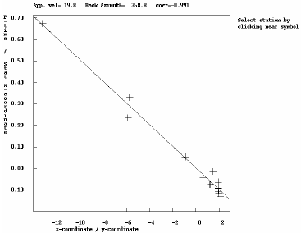
\includegraphics[width=0.9\linewidth]{fig/fig5}}
\caption{The linear fit of P-arrival times to a plane wave. 
For more details, see \citet{havskov2010}.}
\label{fig:pfit}
\end{figure}

PUT: Register event. This option is mainly meant to be used with the SEISNET data collection system. The command cleans up the S-file for all SEISNET operations. It removes commented out ID-lines and copies the waveform files given for the event from the current directory to WAV. The command is equivalent to the register command in MULPLT. If events are auto registered with AUTOREG, the command can be used to clean up and inspect incoming data without using MULPLT directly. 

PMAC: Windows only program PROMAC for processing macroseismic information to calculate intensities from felt information and model the macroseismic intensities. The program can also plot associated pictures (in directory PIC). All information is stored in the S-file. The program was written by Bladimir Moreno, and has a separate manual, see INF directory. Program must be installed separately, zip file in SUP. 

P: Plot event with \index{MULPLT}\index{Plotting traces}MULPLT 

PO: Use MULPLT with defaults. This means that no questions will be asked and the plot appears in multi trace mode with default channels and default filters as given in the \texttt{MULPLT.DEF} file in DAT. Useful option for routine inspection of raw data. 

PITSA: Run the \index{Pitsa program}Pitsa program, see section \ref{subs:pitsa} (Not on PC).

PRINT: The current S-file is printed on the default printer, to set up printer command, 
see \texttt{SEISAN.DEF} (section \ref{sect:seisan.def}). 
\index{Print S-file}\index{EEV print command}\index{S-file, print} 

Q: Quit EEV 

REG: Same as PUT. 

R: \index{Rename event type}Rename event type - Giving an event a new type requires changing the header in the S-file and the S-file name. All this is done with R-command. You are prompted for a new type (can be the same in which case nothing is done). A new S-file is made and the old deleted. The CAT-file is NOT changed so if no UPDATE is done, the event there will remain with wrong type. Event types are L: Local event, R: Regional event and D: Distant event.  
\index{Change event id}Change events id - By adding a second charater to the event type the event id will be changed too. E.g. changing the event to a local explosion one must type LE. Use LB to replace the E with a blank.  Standard event id's are: E = Explosion, P = Probable explosion, V = Volcanic and Q = Confirmed earthquake

\index{RMSDEP}RMSDEP: Calculates and plot\index{Depth as function of rms}s \index{RMS as a function of depth}RMS as a function of depth for current event. 
%\textcolor{red}{jh-change: 
Note: Program starts by reading STATION0.HYP so if current events 
uses e.g. STATION1.HYP, STATION0.HYP must be there also. 
% jh-change, following do not seem to be the case: RMSDEP also operates as a freestanding program with additional capabilities, see description in program. 

SAC: Convert all data to SAC format and starts the SAC processing system ( not distributed with SEISAN, must be obtained separately), not on PC. 

Sxxxxxx: \index{Search}Search for next pairs of events separated in time by xxxxxx secs (max 999999). If no value is given, 180 secs\index{Associate events in time} is used. The command is intended for finding events to be merged after putting together two different data sets with SPLIT. If a new time instead of the default 180 is entered, it will remain in effect for the whole 

EEV session. NOTE, that the search starts with the current event, so after using S, one return to go to the next event must be given to start a new search. 

SS: Find next unprocessed event in database. Events, which have status in ID line as follows: SPL: split with SPLIT program, HYP: auto-located with HYP, NEW: new event from EEV or ARG: registered by AUTOREG. The idea is that when new unprocessed data have entered the database by one of these programs, it should be easy for the operator to find the event. In EEV, an N near the end of the prompt line indicates an event with this status. 

T: Type event. 

TT: Type only header of event. 

%\textcolor{red}{lo-change:
\index{TTPLOT}
TTPLOT: The program reads P and S-arrival times from S-file and makes a
travel time plots. The program 
is useful for checking readings, see section \ref{subs:ttplot}. The 
lines connect the computed first arrivals for P and S, respectively.

UPDATE:\index{UPDATE} Updates (overwrite) S-file with hypocenter, 
magnitudes, residuals etc. Note that the CAT file IS NOT UPDATED
\index{Updated S-files}
\index{S-file, update}. 
This can only be done with stand-alone command UPDATE, see section \ref{sect:update-upd}. 

U: Update EEV event list. All S-file names are read in again. Is useful if data arrives during an EEV session, like when using Copy command from another data base. 

USERCOM\index{USERCOM}: Starts user defined program with command 
\texttt{usercom -sfile $<$sfile-name$>$}, where usercom is the command name. 
This command is useful for example if you want to start your program 
to create a report based on the S-file, from EEV. Note: the usercom 
is not a SEISAN program. 

W: Check if event has waveform files. If so, check in which directory 
they are if present on the system. The search will start in current 
directory, then WAV followed by all directories defined with keyword 
WAVEFORM\_BASE in \texttt{SEISAN.DEF} in DAT. 

WAD: The program  reads the data for the event and then asks if all phases are going to be used or only phases of the same type like Pg and Sg. Ideally, only phases of the same type should be used, however in practice it might be interesting so see all data, it might give an idea about phase identification. The Wadati parameters will now be calculated and shown on the screen. Optionally a plot can now be made. The plot shows the Wadati diagram. On the left is shown all stations with corresponding S-P times. Any station on the plot can be identified with the cursor. Point the cursor near a symbol and click and the station data will be shown in the upper right hand corner. This facility is used to identify bad picks. The plot output file is called \texttt{wad\_plot.eps}.\index{Wadati} 

Z: \index{Automatic phase picking}Automatic phase picking. A waveform file 
must be present. See also the AUTO program section \ref{sect:auto-p-pick}. 

Below is shown a session with EEV on PC.  

Example of using EEV for November 1993 

\begin{boxedverbatim}
eev 199311

1993 11 Reading events for base AGA          18
#    1  2 Nov 1993 17:06 48 L   60.443    4.512  2.0  1.5 N 1.8CBER    6  ? 
#    2  5 Nov 1993 22:37 21 D                                          1  ? 
#    3  5 Nov 1993 22:37 23 D                                          1  ? 
#    4  5 Nov   93 22:39  2 L                                             ? 
#    5  5 Nov   93 22:40 58 L                                             ? 
#    6  7 Nov 1993 23:40 43 L   67.837   20.059 15.0  0.7  2.5CBER     7  ? 
#    7  7 Nov 1993 23:43 17 L   66.307    6.919 31.0  1.4  3.1CBER     8  ? 17
#   17 19 Nov 1993 01:45 29 D   70.069  139.780   .1  0.1              7  ? t
 
File name: \seismo\REA\AGA__\1993\11\19 0145-29D.S199302                                         
1993 1119 0145 29.0 D  70.069 139.780   .1  BER  7  .1                        1
                .19     999.9   821.9999.9   .3206E+06   .2536E+07   .2639E+08E
ACTION:UPD 97 03 25 21:28 OP:jh   STATUS:               ID:19931119014529     I
93111901.K41                                                                  6
  93 1119  153  6.5 D                                                         1
9311 19 0153 06S.NSN_09                                                       6
STAT SP IPHASW D HRMM SECON CODA AMPLIT PERI AZIMU VELO SNR AR TRES W  DIS CAZ7
KBS  SZ EP        151 54.8                                     13.4 0 3365 161 
TRO  SZ EP        153 03.0                                       .010 4420 169 
MOL  SZ EP        153 50.51                                      .010 5070 165 
ASK  SZ EP        154 04.0                                       .010 5262 164 
BER  SZ EP        154 05.0                                       .110 5274 165 
EGD  SZ EP        154 05.5                                       .110 5285 165 
KONO BZ EP   9    153 49.21                                    25.5 0 5413 167 
                                                                               

#   17 19 Nov 1993 01:45 29 D   70.069  139.780   .1                     7  ? 
#   18 21 Nov 1993 01:53 56 L   60.184    4.965 15.0  N 0.5  2.6CBER    11  ? 
 1993 11 Reading events for base AGA          18
    1  2 Nov 1993 17:06 48 L   60.443    4.512  2.0     2.2  1.8CBER     6  ? q
\end{boxedverbatim}


In the above example (PC), the month has 18 events. For each event, vital information is displayed: Date, type, hypocenter, RMS, first magnitude and number of stations (number in S-file which might be larger than number used for location as given in S-file header line after a location). In this way the user can quickly search for events wanted and get important information without looking at all the details. The first event in the list is newly entered into the database as indicated with the N near the end of the line. In the above example, a return was made to go to next event until event \#7 after which a jump was made to event 17. For this event, all parameter data was displayed with the 't' command. A return was made to event 18, another return and the event list was read in again and event \#1 again became the current event. Note that not all events had a location. 

Below are shown examples of the commands (C)opy, (D)ate, a(S)sociate and (A)ppend. Comment are preceded by '!' and written in bold. The database is EAF. 

\begin{boxedverbatim}
EEV 199405 EAF

1994  5 Reading events for base EAF         613   ! the month has 613 events
#    1  1 May 1994  1:18  8 D                                               ? 
#    2  1 May 1994 11:37  6 L                                               ? 
#    3  1 May 1994 12:00 33 D   36.607   68.449 15.0  2.4    ! go to day 20 ? d20
#  366 20 May 1994  5: 2  8 R                                               ? c
                                                ! copy an event to working dir.
 Copy event: Other database, give 1-5 letter name
             Working directory in file eev.out: return

#  366 20 May 1994  5: 2  8 R                                              ? 
#  367 20 May 1994 10:59 32 D      ! jump to 530                           ? 530
#  530 26 May 1994  8:55 11 D      ! look for time association             ? s
 
  549 27 May 1994  9:27 41 L                                        Associated
  548 27 May 1994  9:27  1 L       ! append to next event            ? aa
 Event #  549 appended to event #  548   Appended event still present
 Do you want to delete appended event(y/n=return)y   ! delete appended event

Backup copy saved as: \seismo\REA\DELET\1994\05\27 0927-41L.S199405 ! del. ev. save   
Deleted file          \seismo\REA\EAF__\1994\05\27 0927-41L.S199405 ! app.ev. del.
1994 05 Reading events for base EAF         612    ! event list updated
#  548 27 May 1994  9:27  1 L                     ! jump to 222            ? 222
#  222 12 May 1994 23:28 10 L                     ! change event type      ? r
 
 Change event type to L,R or D ?r

New file       \seismo\REA\EAF__\1994\05\12 2328-10R.S199405      
Deleted file:  \seismo\REA\EAF__\1994\05\12 2328-10L.S199405    
Reading events for base EAF         612
#  222 12 May 1994 23:28 10 R                                        ? 
#  223 13 May 1994  1: 1 37 L                                        ? 
#  224 13 May 1994  1:16 44 L                                        ? q

Stop   Program terminated.\end{boxedverbatim}


*************************************************************************** \newline
When the interactive location is finished, the database should 
be \index{UPDATE}updated, see section \ref{sect:hypocenter}. \newline
*************************************************************************** \newline

Using EEV on a subset of events or using alternative databases: 

Since the EEV procedure or the HYP program will work on an \index{Index file}index file, the user can create a subset of his own interesting events to work with by creating his own index file with just these events. The \index{Local index file}\index{Index file}index file can be created by searching through the database using SELECT or it can be created manually with the C-command in EEV. 

Local database: 

If data is extracted by using the COLLECT or \index{SELECT}SELECT and then split up again using SPLIT, it is possible to keep all files in a working directory by not specifying database when splitting up. Another simple way is to use the Copy function in EEV and copy directly from a named data base to the local data base. Programs will then look for S-files in the current directory instead of in the database. 

In addition to working with index files, there is also the possibility of storing data in \index{Different databases}different databases. By default, the data is always stored in BER. However, the user can also create another \index{Database structure}database structure (file structure) with another name and programs and procedures will work on that database too. There are some restrictions: The new database, which is a subdirectory under SEISMO/REA, just like BER, MUST have a 1-5 letter name. Currently, the alternative database is used in our Institute to store data from other agencies like NAO, which in some cases are copied to our own database (C-command under EEV).  The name DELET is reserved for the \index{DELET database}DELET database, which is always present. 

%\textcolor{blue}{lo-comment: remove next version}
%\subsection{EEV driver program: JSEISAN}
\index{JSEISAN} 

Software and manual by Bladimir Moreno 

JSEISAN is a JAVA application for providing a user-friendly graphical interface of some of the functions of the SEISAN earthquake analysis system. The program uses the functions implemented in SEISAN by executing external commands, which mean that most of the data processing is performed with the SEISAN software. JSEISAN is mainly a tool for formatting the input data and display the results. The program was developed with Visual Cafe 4 Standard Edition. The software operates in Unix and Windows environments. 

Using JSEISAN 

The program is started by giving command jseisan and the window 
(Figure \ref{fig:jseisan}) below will appear. 

\begin{figure}
\htmlimage{scale=2.0}
\centerline{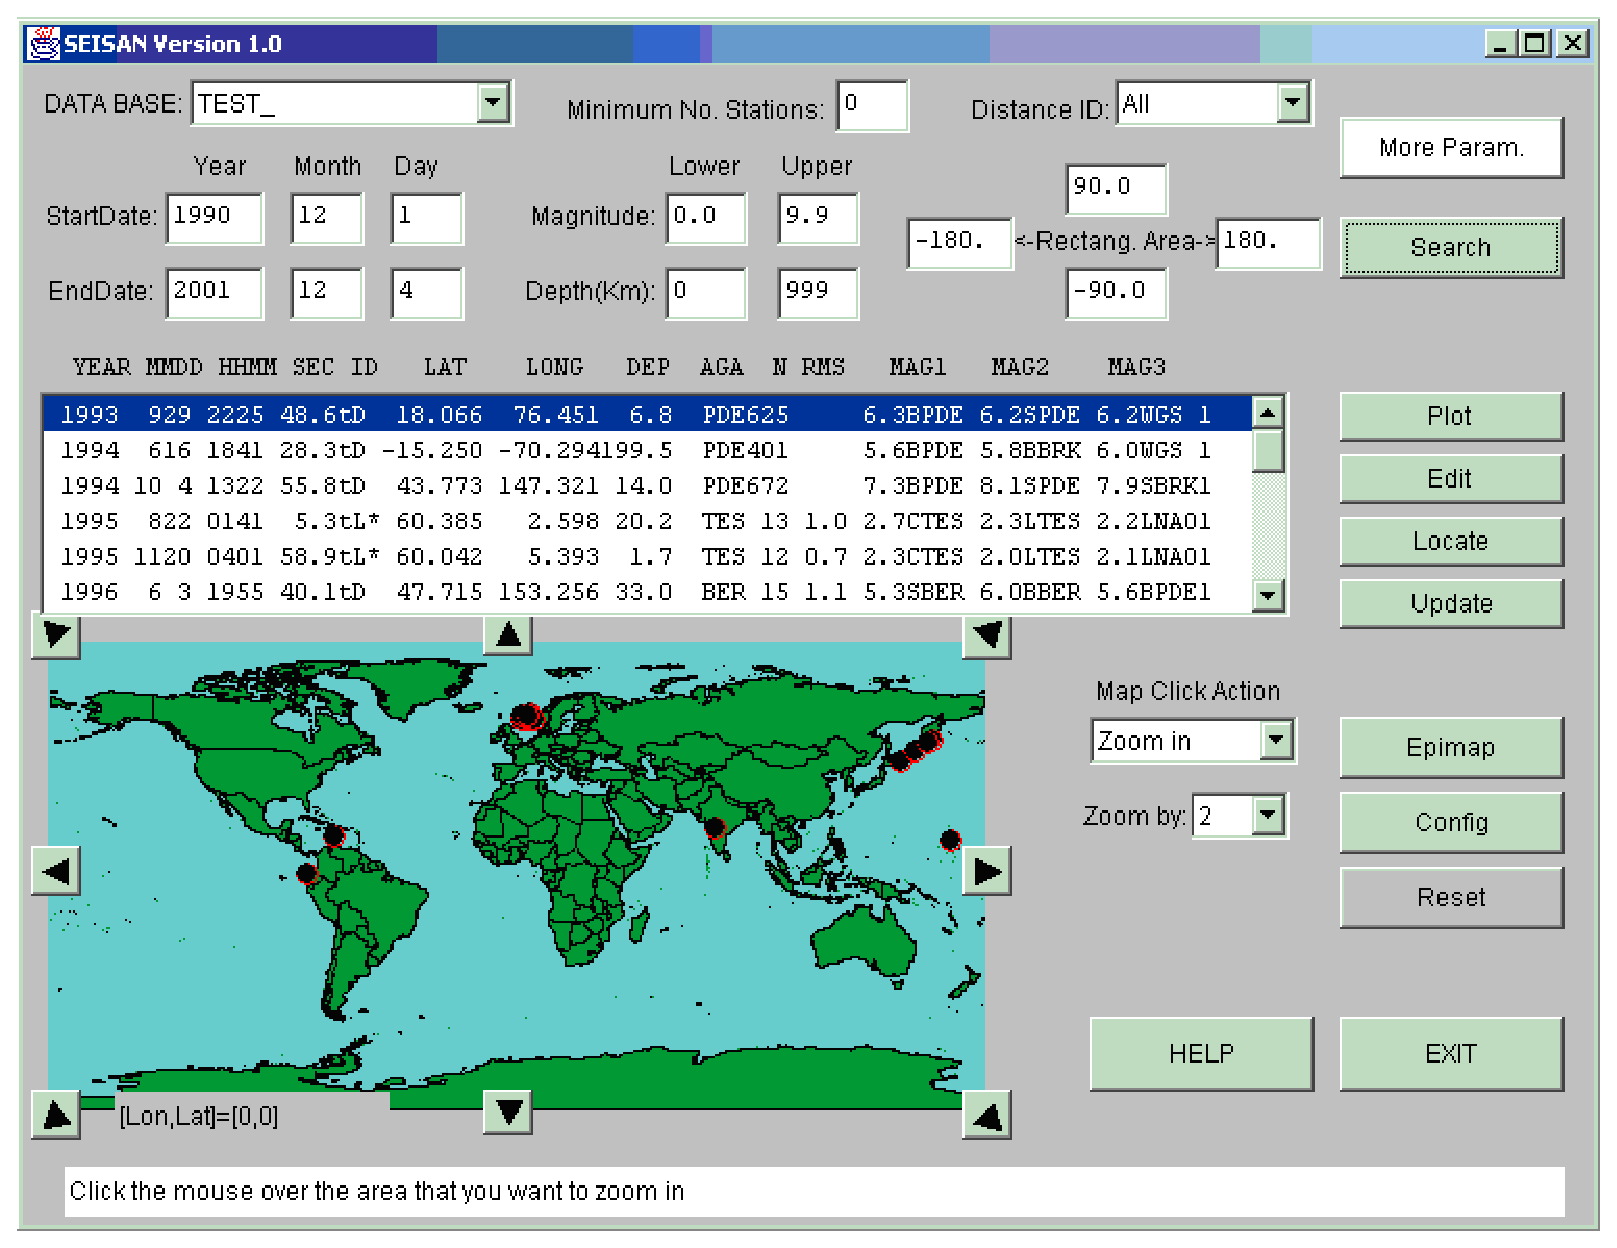
\includegraphics[width=0.9\linewidth]{fig/fig6}}
\caption{Main window of JSEISAN.}
\label{fig:jseisan}
\end{figure}

The user interaction with JSEISAN can be classified as: (1) Searching for earthquakes and (2) working with a particular earthquake. It is assume that a standard SEISAN data base is available with S-files and CAT files in the CAT directories (see SEISAN manual). The interface has a main window where the user can search earthquakes ($<$Search$>$ button) set up by a range of values 
(Figure \ref{fig:jseisan-Dialog-window}). 
As a result of the searching process, an earthquake list is shown on the screen and a set of functions is offered. In addition, the epicenters of the earthquake list are plotted on the map. Because there is a direct link between the map and the list, the selected earthquake is highlight on both the map and the list when the user is navigating either through the list or through the map (\textbf{see Interactive mapping tool}). 

Configuring JSEISAN 

JSEISAN \index{JSEISAN, configure}has several configuration variables to be set up by the user. In order to configure the variables, you have to click the button $<$Config$>$ (Figure \ref{fig:jseisan}). The configuration parameters are stored in the file \texttt{SEISAN.DEF}. \index{SEISAN.DEF}The editing process of this file is performed through the JAVA program \texttt{SEISCONF.class} (see SEISCONF). A complete description of the configuration parameters is given in at the end of this section. 



\textbf{Selecting the database to work with}

The desired SEISAN database is selected from the combo-box labeled as ``DATA BASE'' located in the left upper part of the main window (Figure \ref{fig:jseisan}). The last item in the combo-box corresponds to a SEISAN CAT file labeled as ``USER FILE''. When this item is selected, the user can load a file, for example \texttt{collect.out}, to work with. 

\textbf{Searching}

\index{Searching in the data base}
There are two windows for setting the parameters used in the searching process: (1) A main window, which contains the most common parameters (Figure \ref{fig:jseisan}) and 
(2) 
A second window (Figure \ref{fig:jseisan-Dialog-window}) which contain the rest. This second window is opened by clicking the button $<$More Param.$>$. In order to perform the search you have to: 

\begin{enumerate}
\item Set up the parameters (period of time, magnitude range, geographic area, etc.) needed in the searching process. 
\item Click the button $<$More Param.$>$ for refining the searching process (if needed). A dialog-box (Figure \ref{fig:jseisan-Dialog-window}) for setting the additional parameters is shown. 
\item Press the $<$Search$>$ button. 
\end{enumerate}


\begin{figure}
\htmlimage{scale=2.0}
\centerline{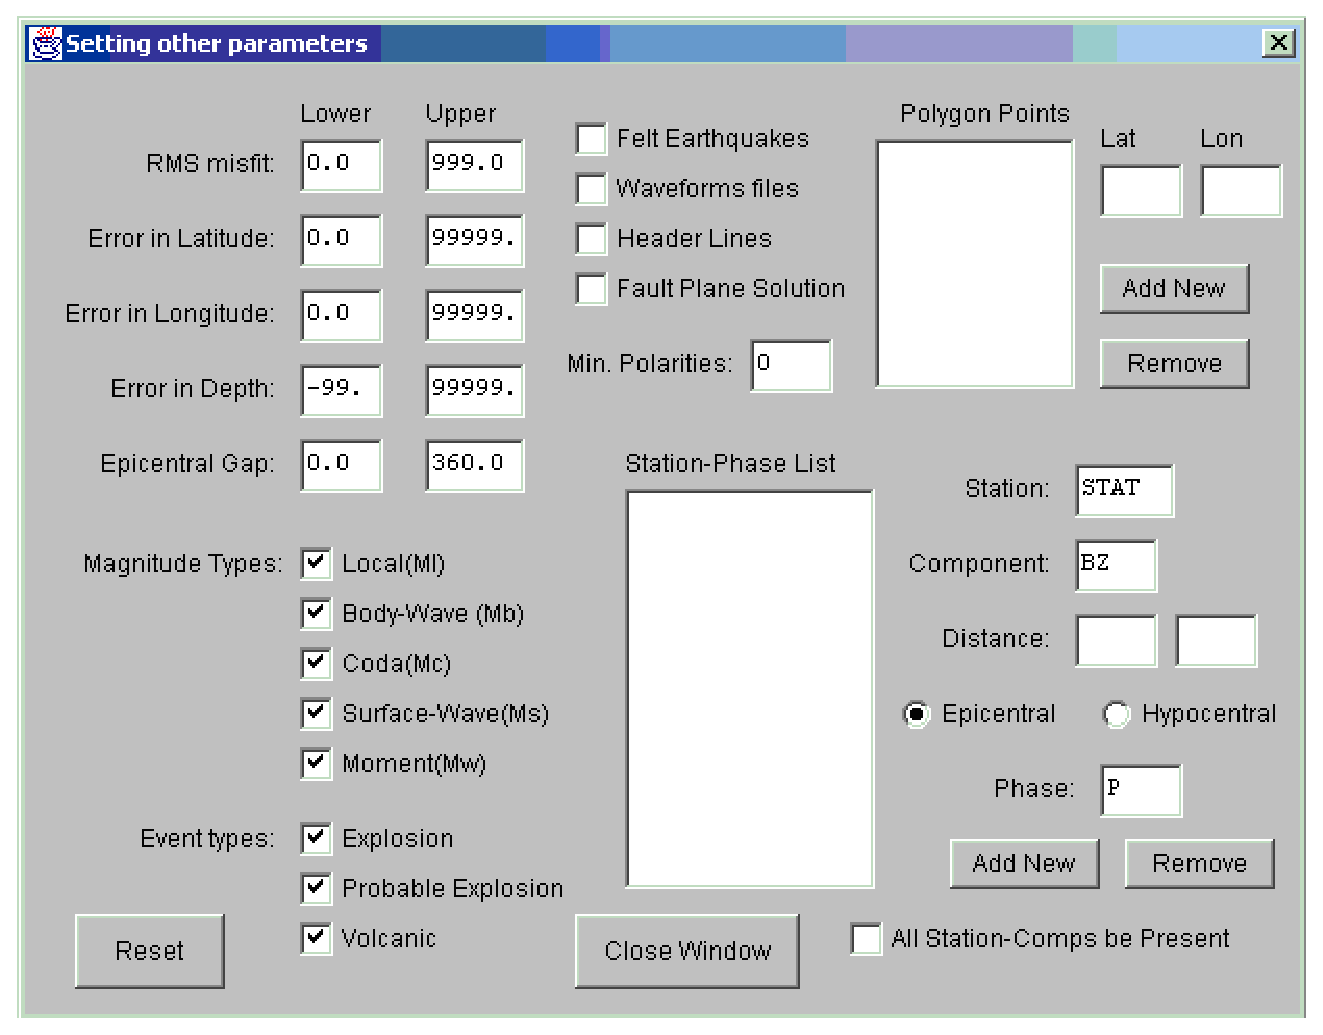
\includegraphics[width=0.9\linewidth]{fig/fig7}}
\caption{Dialog-window for setting other parameters used during search.}
\label{fig:jseisan-Dialog-window}
\end{figure}

Interactive Mapping Tool 

Figure \ref{fig:jseisan} shows a map with the locations of the earthquakes obtained during the searching process. The map has an equidistant cylindrical projection, which means that one unit of longitude has the same distance to one unit of latitude. This map can be used as interactive mapping tool. For this purpose, 4 options are included in the combo-box labeled as ``Map Click Action'' (Figure \ref{fig:jseisan}). The options are ``Select'', ``Zoom in'', ``Zoom out'' and ``Polygon''. The function of each radio-button is as follows: \index{MAP} 

``Select'': When it is active, the user can click over the circle identifying the location of the earthquake. The associated earthquake in the list will be highlighted. 

``Zoom in'': When it is active, the user can zoom in the map by a factor of 2,4,8,16 or 32. The zoom factor is selected from the combo-box labeled as ``Zoom by''. The clicked point on the map will be the center of the new map. \index{SELECT}\index{Zoom in map} 

``Zoom out'': Similar to ``Zoom in'' but with reverse effect. 

``Polygon'': When it is active, the user can define the points of a polygon by clicking on the map. The polygon is closed when a click over the starting point is made. Once the polygon is defined, the user can edit its points by using the refined search window, which is reach by clicking the $<$More Param.$>$ button. Epicenters inside the polygon can now be selected with the search function. \index{Polygon, select in} 

The zoomed map is taken either from Internet or locally. In the case of being retrieved locally, the images are taken from the directory specified by the configuration variable \textbf{IMGMAP\_PATH}. The images are saved in sub-directories according with the level of zoom. For example in case of 6 levels of zoom you will find the directories ZOOM0, ZOOM1, ZOOM2, ZOOM3, ZOOM4, ZOOM5 and ZOOM6. ZOOM0 only has one image, the whole world. ZOOM1 contain 9 images, the world is divided into 9 equal areas. ZOOM2 contain 81 images, the world is divided into 81 areas and the last 
6
level of zoom (ZOOM6) contains $9^{6}$ images. The image files are numbered as IMG\#.gif from left-up to right-down, like a matrix but using only one index. When the map is being retrieved from Internet there is no zooming limitation. You can go as deep as you want. The configuration variable \textbf{MAP\_SERVER} controls where to retrieve the image from. 

\textbf{Making an epicenter map from the earthquake list}

An epicenter map can be made through the SEISAN command ``EPIMAP''. The steps are:  \index{EPIMAP} 

\begin{enumerate}
\item Press the $<$Epimap$>$ button 
\item A new dialog-box for the configuration of the map is shown 
(Figure \ref{fig:jseisan-Dialog-box}), then click the  $<$Ok$>$ button. 
\end{enumerate}

\begin{figure}
\centerline{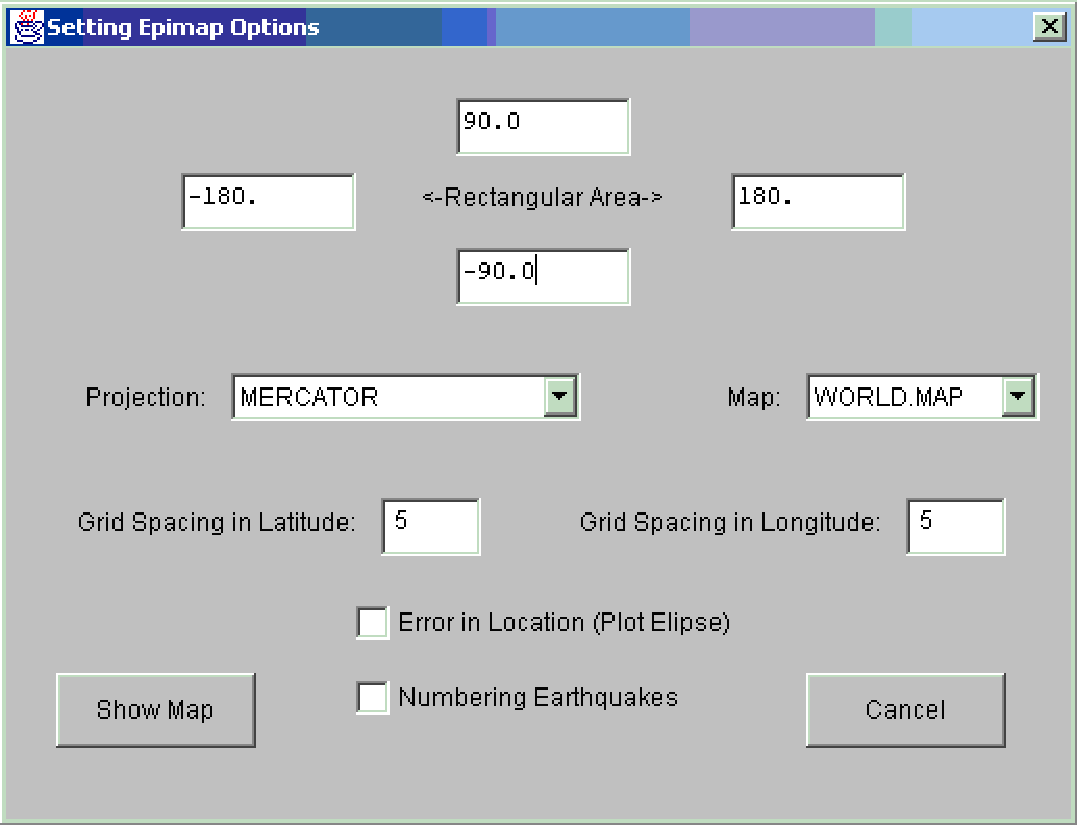
\includegraphics[width=0.9\linewidth]{fig/fig8}}
\caption{Dialog-box for setting the EPIMAP input data. Only the most common EPIMAP parameters are set.}
\label{fig:jseisan-Dialog-box}
\end{figure}

\textbf{Working with a particular earthquake}\newline
There are four available options for working with a particular earthquake of the list: (1): Plot waveforms, (2) Edit phases, (3) Locate and (4) Update. The associated buttons are located on the right side of the earthquake list (Figure \ref{fig:jseisan}). 

\textbf{Plotting and processing traces}\newline
Any number of channels, up to 75, can be plotted. In order to visualize a large number of channels, a page system is implemented, when more than 12 channels are selected. For practical reason, two operation modes are given in the plotting process: 
``multi-traces mode'' (Figure \ref{fig:jseisan-Multi-Trace-mode}) and ``single-trace mode'' 
(Figure \ref{fig:jseisan-Single-Trace-mode}). 
The distinction is made mainly for choosing which channels will be plotted together (multi-trace mode with select/unselect) and to navigate through the selected channels in more detail (single-trace mode). This is similar to MULPLT in SEISAN. In both operational modes, picking phases, zooming and filtering can be done. For ``multi-trace mode'', a set of additional options are available, e.g. save traces, which is applied to the plotted channels on the screen within a selected time window. 

\begin{figure}
\htmlimage{scale=2.0}
\centerline{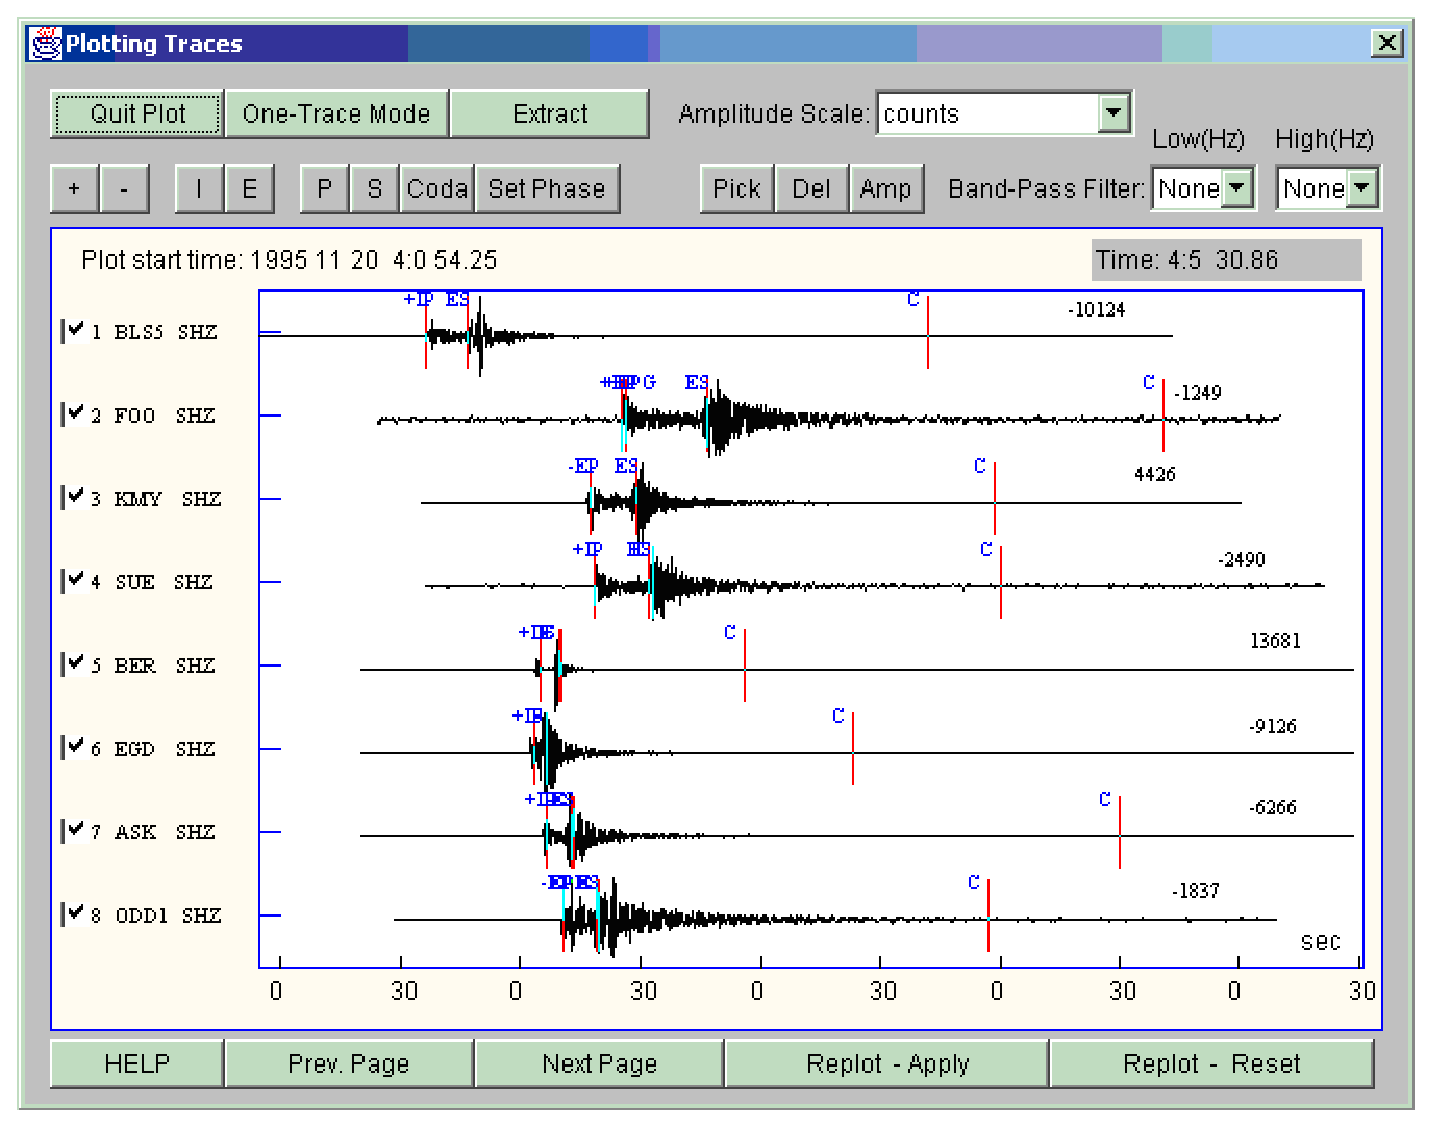
\includegraphics[width=0.9\linewidth]{fig/fig9}}
\caption{ Plotting window. Multi-Trace mode.}
\label{fig:jseisan-Multi-Trace-mode}
\end{figure}

\begin{figure}
\htmlimage{scale=2.0}
\centerline{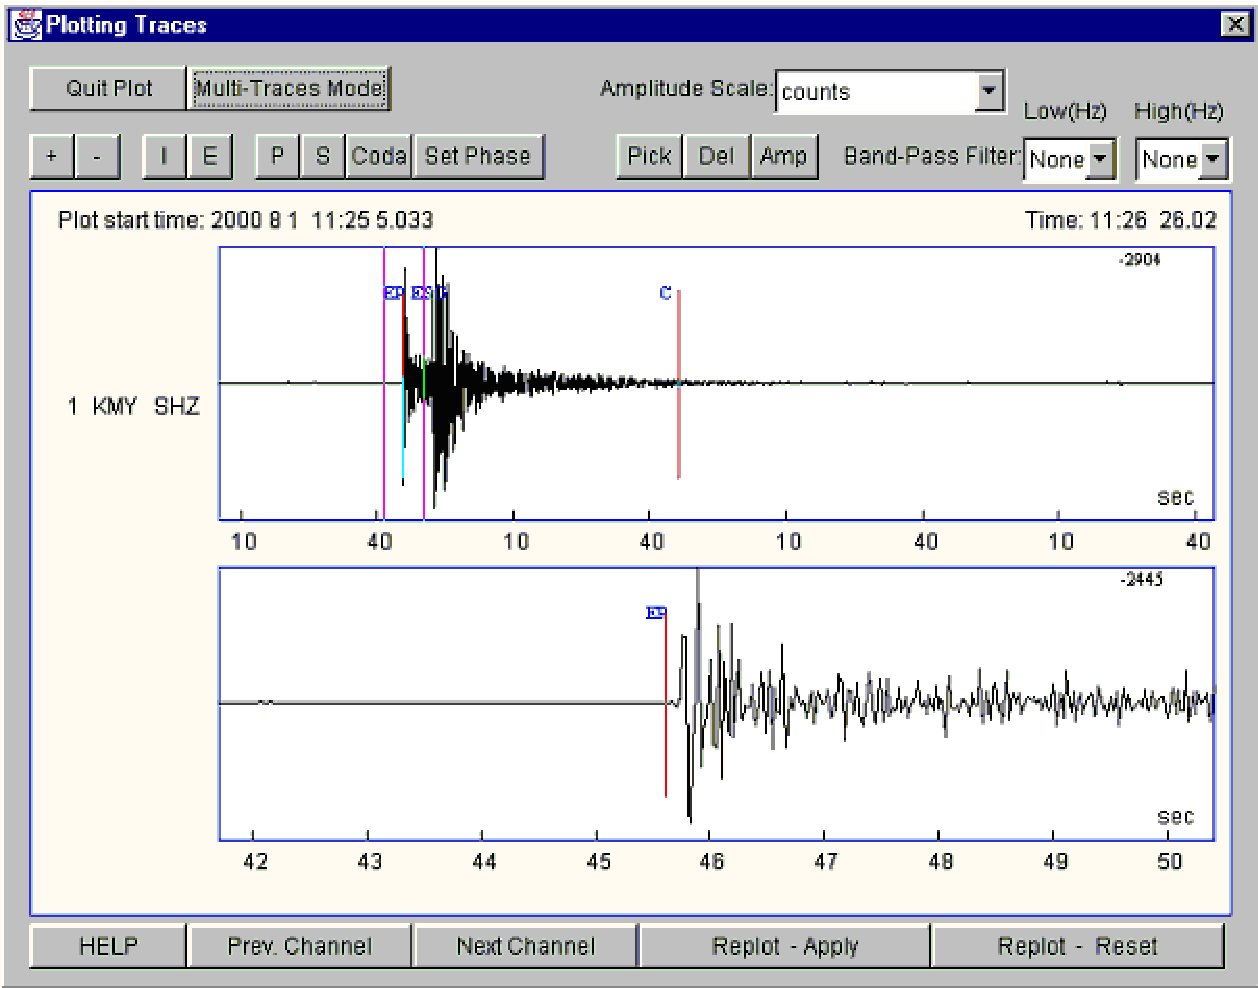
\includegraphics[width=0.9\linewidth]{fig/fig10}}
\caption{ Plotting window. Single-Trace mode.}
\label{fig:jseisan-Single-Trace-mode}
\end{figure}

The steps to plot a particular earthquake selected from the list are: 
\begin{enumerate}
\item Select a desired earthquake from the list by clicking the left button of the mouse on it (Figure \ref{fig:jseisan}). 
\item Press the $<$Plot$>$ button. 
\item A new dialog-box for the selection of the channels to be plotted is shown (Figure \ref{fig:jseisan-Selection-of-channels}), then click the $<$Plot$>$ button. 
\end{enumerate}

\begin{figure}
\htmlimage{scale=2.0}
\centerline{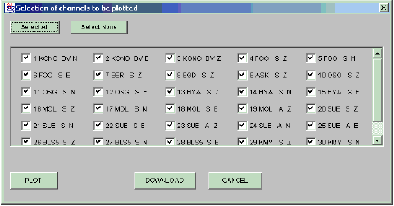
\includegraphics[width=0.9\linewidth]{fig/fig11}}
\caption{Selection of channels.}
\label{fig:jseisan-Selection-of-channels}
\end{figure}

Filtering one/several channels 
\begin{enumerate}
\item Select the low corner frequency of the Band-Pass filter (select ``none'' if a High-Pass filter is desired) from the combo-box labeled as ``Band-Pass filter'' 
(Figure \ref{fig:jseisan-Multi-Trace-mode}).  
\item Select the high corner frequency of the Band-Pass filter (select ``none'' if  a Low-Pass filter is desired). 
\item Make a zoom over the traces (\textbf{see Zooming section}) or click the button $<$Replot - Apply$>$\index{Zoom in JSEISAN} 
\end{enumerate}

\textbf{Instrument corrections}\newline
Converting the amplitude of one/several\index{Response removal} traces into ground velocity, displacement or acceleration and simulating Wood-And., Mb and Ms amplitude. 

\begin{enumerate}
\item Select the desire amplitude from the combo-box labeled  ``Amplitude Scale'' 
(Figure \ref{fig:jseisan-Multi-Trace-mode}). 
\item Make a zoom over the traces (\textbf{see Zooming section}) or click the button $<$Replot - Apply$>$ 
\end{enumerate}

\textbf{Picking and removing phases}\newline
\index{Phase picking} 
\begin{enumerate}
\item
 Press the $<$+$>$/$<$-$>$ button (Figure \ref{fig:jseisan-Multi-Trace-mode}) 
in order to select/unselect the polarity (Compression/ Dilatation) of the first impulse (if needed) 
\item Press the $<$I$>$/$<$E$>$ button in order to select/unselect the shape (Impulsive/Emergent ) of the first impulse (if needed) 
\item Press the button identifying the phase to be picked/removed ($<$P$>$/$<$S$>$,\dots ) 
\item Press the $<$Pick$>$/$<$Del$>$ button to active the picking/deleting process 
\item Move the mouse pointer to the position of the first impulse 
\item Click the left button 
\end{enumerate}


* The previous buttons will be kept active. Furthermore you can pick the selected phase for the rest of the channels without going through the first 4 steps. 

Reading amplitude \newline
\begin{enumerate}
\item
 Press the $<$Amp$>$ button (Figure \ref{fig:jseisan-Multi-Trace-mode}) 
to active the reading process 
\item Move the mouse pointer to the position of one extreme (upper or lower) of the signal    
\item Click the left button (a horizontal line will be drawn) 
\item Move the mouse pointer to the position of the opposite extreme of the signal one half period away.  
\item Click the left button 
\end{enumerate}

* The $<$Amp$>$ button will be kept active. Furthermore you can continue reading amplitudes for the rest of the channels without going through the first step. 

Zooming \newline
\begin{enumerate}
\item
 Move the mouse pointer to the initial time of the zooming window (the time is shown above the right-upper-corner when you move the mouse) 
\item Click the left button 
\item Move the mouse pointer to the final time of the zooming window 
\item Click the left button 
\end{enumerate}


Extracting traces from a time window \newline
You can extract either raw or processed traces from the plotting window 
(Figure \ref{fig:jseisan-Multi-Trace-mode}). The steps are: 

\begin{enumerate}
\item
 Select/unselect (see ``Other options'' section) the channels to be downloaded  
\item Make any desire processing (zoom, filter, etc.) if you want to save  processed traces or a data selection of the original traces. 
\item Press the $<$DownLoad$>$ button. \index{Extract data in JSEISAN} 
\end{enumerate}


The data will now be stored in your working directory in SEISAN format in a file with name specified by the user. Since an integer format is used, processed data with amplitudes less than 1 will have amplitude values 0. 

Other options 

Switching between ``single'' and ``multi'' traces mode 

\begin{enumerate}
\item
Press the $<$single-trace mode$>$/$<$multi-traces mode$>$ button 
(Figure \ref{fig:jseisan-Multi-Trace-mode} and Figure \ref{fig:jseisan-Single-Trace-mode}). 
\end{enumerate}

Show/hide channels to be plotter together on the screen 

\begin{enumerate}
\item
 Press the $<$Replot - Reset$>$ button (Figure \ref{fig:jseisan-Multi-Trace-mode}) 
\item
 Click the left button of the mouse over the check-box identifying each channel in order to select/unselect the channel 
\item
 Press the $<$Replot - Apply$>$ button 
\end{enumerate}


Navigating through individual channels \newline
\begin{enumerate}
\item
 Go to the ``single-trace'' mode (Figure \ref{fig:jseisan-Single-Trace-mode}). 
\item
 Press the $<$Next Channel$>$ button to go forward or $<$Previous Channel$>$ to go backward 
\end{enumerate}


Navigating through pages of channels (12 channels as maximum on one page) \newline
\begin{enumerate}
\item
 Go to the ``multi-trace'' mode (Figure \ref{fig:jseisan-Multi-Trace-mode}) 
\item
 Press the $<$Next Page$>$ button to go forward or $<$Previous Page$>$ to go backward 
\end{enumerate}


Editing S-files\newline
The editing window (Figure 
\ref{fig:editing-window}
) has 3 buttons for closing the window. When you click the button $<$Save \& Exit$>$ the S-file is physically modified on the hard disk. The $<$close$>$ button keeps the changes in memory until another earthquake is selected on the list. So, you can still perform full processing without making any real change in the S-file. The steps to edit the S-file are: 

\begin{enumerate}
\item
 Select a desired earthquake from the list clicking the left button of the 
mouse on it (Figure \ref{fig:jseisan})
\item
 Click the $<$Edit$>$ button 
\item
 An editing window with the information is shown (Figure \ref{fig:editing-window}).
\end{enumerate}

\begin{figure}
\htmlimage{scale=2.0}
\centerline{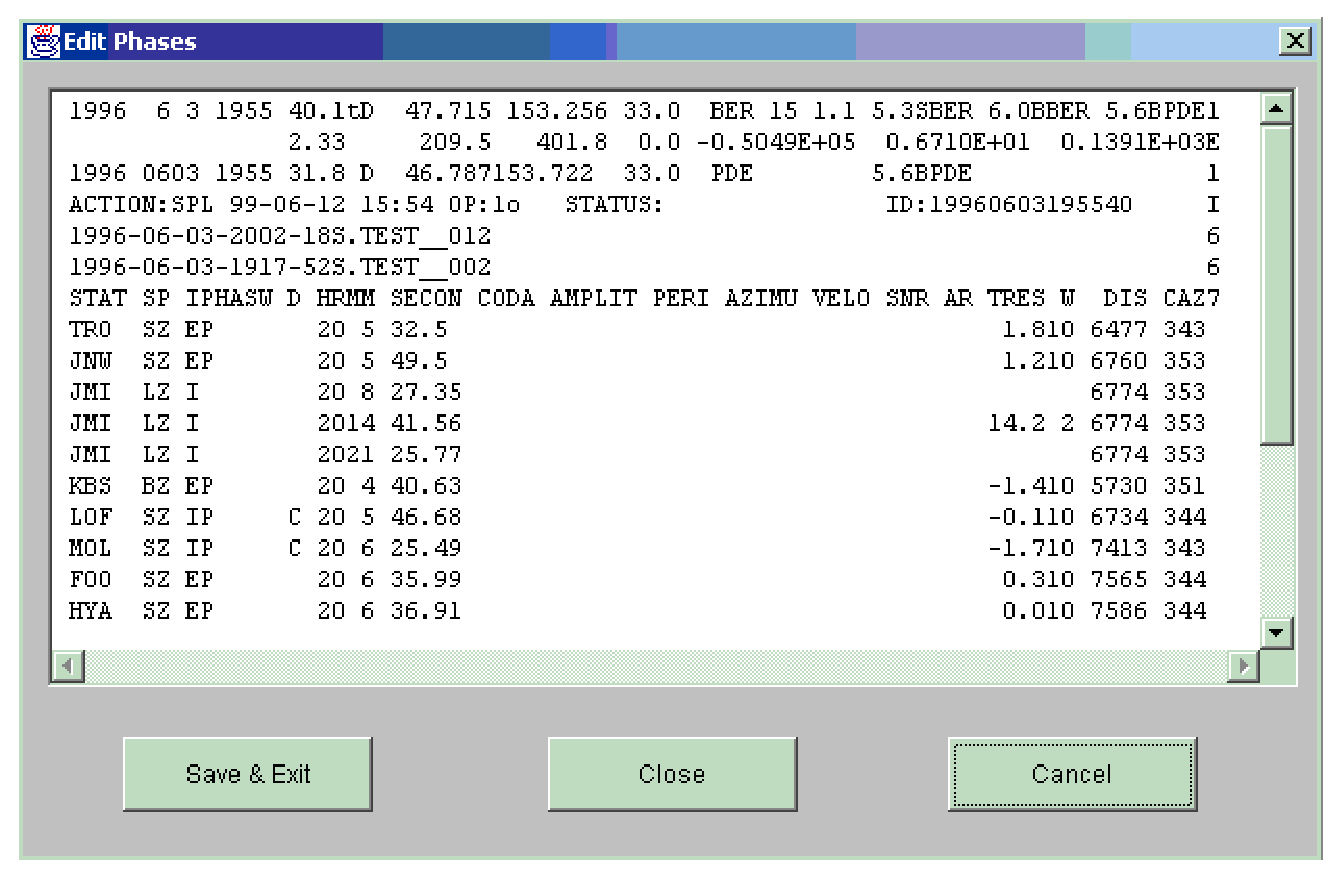
\includegraphics[width=0.9\linewidth]{fig/fig12}}
\caption{Editing window.}
\label{fig:editing-window}
\end{figure}

Note that this editing function do not yet, as in SEISAN EEV, check the file for correct editing. 

Determining hypocenter and magnitude \newline
\begin{enumerate}
\item
 Select a desired earthquake from the list clicking the left button of the mouse on it 
\item
 Press the $<$Locate$>$ button 
\item
 A new window with the results is shown (Figure \ref{fig:hypocenter-determination}) 
\end{enumerate}

\begin{figure}
\htmlimage{scale=2.0}
\centerline{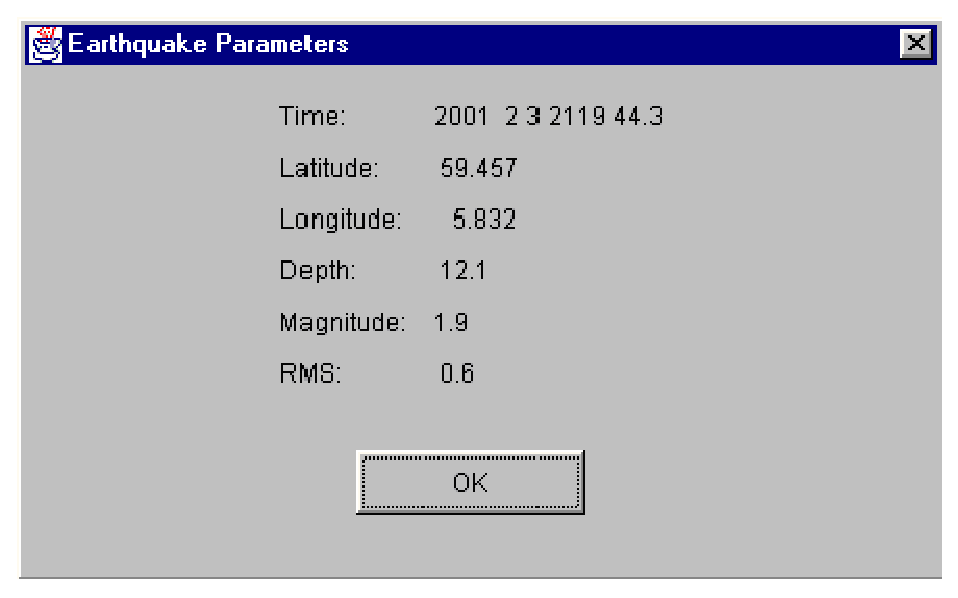
\includegraphics[width=0.9\linewidth]{fig/fig13}}
\caption{Results of the hypocenter determination.}
\label{fig:hypocenter-determination}
\end{figure}

The usual SEISAN files print.out and hyp.out are generated (see section 6.1.1).


Updating the earthquake in the database 

\begin{enumerate}
\item
Select a desire earthquake from the list by clicking the left button of the mouse. 
\item
Press the $<$Update$>$ button (Figure \ref{fig:jseisan}) 
\end{enumerate}

Note: This updates the S-file, but the original CAT file in the database is NOT updated. In order to do so, an update outside JSEISAN must be done (see SEISAN manual). 

Help Function\newline
\index{Help in SEISAN}
The help system implementation is based on PDF files. When the user clicks the $<$HELP$>$ button, a list of PDF files is shown 
(Figure \ref{fig:list-pdf-files}).
The list is stored in the file ``helpmenu.inp'', which is found in the DAT directory. You can edit this file for adding new PDF files to the help system 


\begin{figure}
\htmlimage{scale=2.0}
\centerline{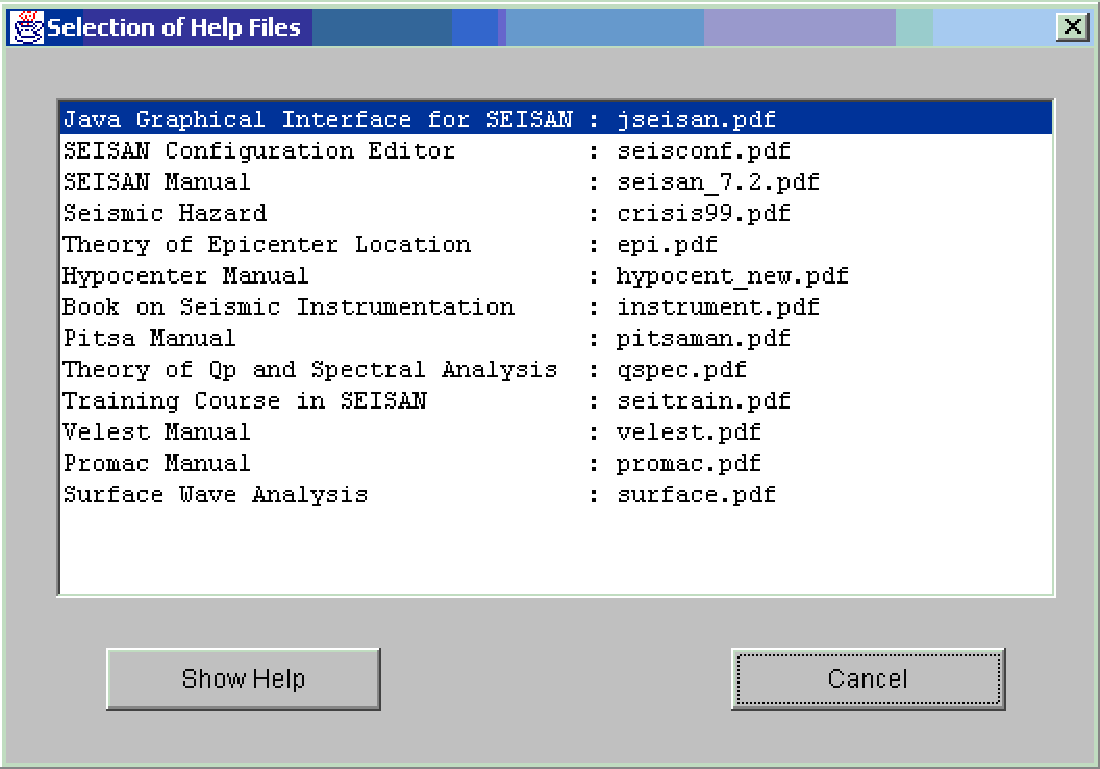
\includegraphics[width=0.9\linewidth]{fig/fig14}}
\caption{Example list of PDF files used for the help system, normally in DAT.}
\label{fig:list-pdf-files}
\end{figure}

\textbf{Configuration parameters in JSEISAN}

\index{SEISAN.DEF}\index{JSEISAN, configuration parameters}The following parameters used by JSEISAN are stored in the configuration file \texttt{SEISAN.DEF}. They can be edited through the program SEISCONF. Most of them are defined to be used only with JSEISAN, but some are already defined in the SEISAN configuration file: \texttt{SEISAN.DEF} ( EPIMAP\_PROJECTION and EPIMAP\_MAP\_FILE) 

\noindent
\textbf{OUTPUT\_DIR}: Output Directory for SEISAN commands results. Default ``./'' \newline
\textbf{EPIMAP\_MAP\_FILE}: Name of the map file for EPIMAP command \newline
\textbf{EPIMAP\_PROJECTION}: Number of the projection for EPIMAP command (see SEISAN Manual) \newline
\textbf{INIT\_IMGMAP\_FILE}: File name of the initial map represented as image. Default ``/seismo/DAT/IMGWORLD.gif''\newline
\textbf{MAP\_SERVER}: Type of map retrieved from Internet or locally; 0: Static local image (country boundaries), 1: Static remote image (country boundaries), 2,3,4,5: Dynamic Remote image (2:country boundaries, 3:Relief from GTOPO30 only land, 4:Two minute shaded relief, 5: Combine 3 and 4). Default 0. \newline
\textbf{IMGMAP\_PATH}: PATH for the static local maps (images) stored in the local hard disk used for zooming. Default ``/seismo/DAT/IMGMAP'' \newline
\textbf{INIT\_MAP\_LOWER\_LATITUDE}: Lower latitude of the initial map. Default -90.0 \newline
\textbf{INIT\_MAP\_UPPER\_LATITUDE}: Upper latitude of the initial map. Default 90.0 \newline
\textbf{INIT\_MAP\_LEFT\_LONGITUDE}: Lower longitude of the initial map. Default -180.0 \newline
\textbf{INIT\_MAP\_RIGHT\_LONGITUDE}: Upper longitude of the initial map. Default 180.0 \newline
\textbf{ACROBAT\_READER}: Path for the Adobe Acrobat Reader (needed for the help files). Default ``/prog/acroread'' for Unix. \newline
\textbf{INTERNET\_BROWSER}: Location and place of browser \newline
\textbf{HELP\_DIR}: Directory of help files, usually INF 



\subsection{EEV Windows driver program: SEISAN} 
\label{subs:eev-win}

The program is an alternative to the standard EEV and it has all the functions of EEV. NOTE, the program has not been updated since SEISAN 8.2.1. The main difference compared to EEV is that is has a 'Windows type' selection of events in the database and that the most used commands in EEV and SEISAN can be executed by pressing a Button. The intention is that the majority of routine tasks in SEISAN can be done within the W95 interface without learning all the SEISAN prompt line commands.  

Starting SEISAN Windows 

When Windows is running, SEISAN can be started by clicking on the SEISAN icon if installed (see section \ref{chap:installation}) or writing SEISAN on the prompt line. SEISAN will start up and show a figure as shown in \index{Windows}
figure 
\ref{fig:windows-seisan-display}.
In addition to the main SEISAN window, there will also be a console window used for input and output since all underlying programs are started from the prompt line. 

Working directory 

Most programs read and write to the current working directory. The name of the working directory is displayed on the bottom of the screen. To change the working directory, press file selection at the top left$�$hand corner. 


% jh change: a new figure should be put in since it has changed
% I have put in a new called figure15.bmp

\begin{figure}
\htmlimage{scale=2.0}
\centerline{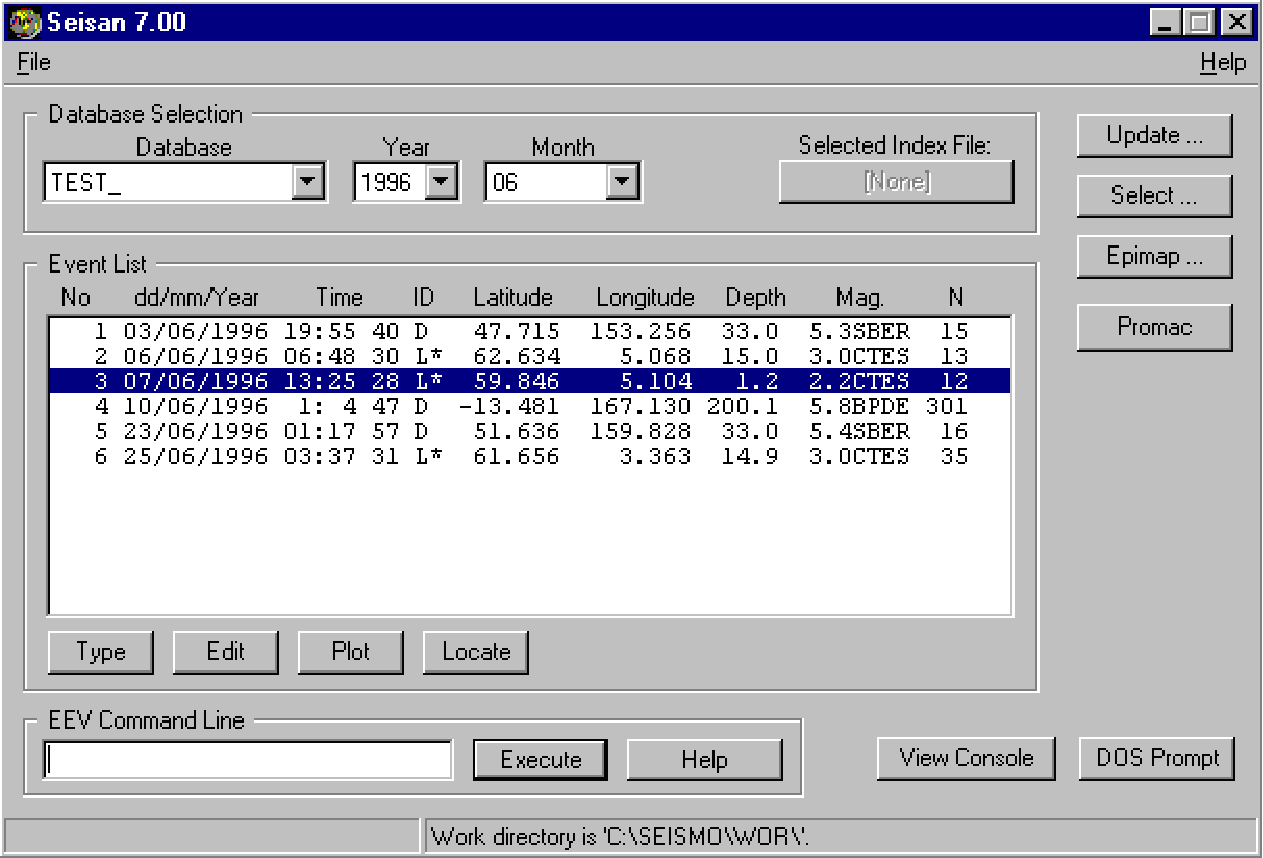
\includegraphics[width=0.9\linewidth]{fig/fig15}}
\caption{Windows SEISAN display.}
\label{fig:windows-seisan-display}
\end{figure}

Database selection 

When SEISAN starts up, it will start with the database used when it last was closed. Other databases can be selected with the 'Database Selection' menu, which also displays the current database. The choices are 

\begin{enumerate}
\item
One of the 1-5 letters databases already in existence. New databases are created as usual with MAKEREA on the prompt line. 
\item
A local database in the current working directory. The current \index{Working directory}working directory is displayed on the bottom of the SEISAN screen. To change the working directory use file selection at the top left hand corner. 
\item
An index file. The file name is selected on the menu 'Selected Index File' 
\end{enumerate}

Year and month selection: If a 1-5 letter database has been selected, the years and months available are seen under year and month buttons and can be selected there. 

Selecting an event 

Once the database has been selected, SEISAN will work much like EEV. The event window will show 12 events with the same information as seen in EEV. The total number of events for the month is shown above the event selection box. The first event in the list will be the current event. Any other event on the list can become the active event by clicking on it and it will be highlighted. Events outside the window can be displayed using the scroll bar. In addition, all EEV commands can be used including event selection commands. This works exactly as in EEV. Write e.g. 22 anywhere on the screen, press return (or click on execute button) and event 22 will be highlighted. 

Commands 

All commands from EEV can be used and they are used like in EEV. Typing e.g. 'l' and return (or click on execute button), will locate the event. While typing the command, it will appear in the 'EEV Command Line' window. The command can be edited and a command can be repeated by just pressing the 'Execute' button or hitting 'return' again. However, the 4 most used EEV commands can also be executed by clicking a command button: 

\noindent
Type: Will display the content of the S-file, same as EEV 'T' \newline
Edit: Edit the S-file, same as EEV command 'E' \newline
Plot: Plot the traces, same as EEV command 'P'. \newline
Locate: Hypocenter location, same as EEV command 'L' 

In addition it is possible to display the S-file header line by double clicking on the active event. This corresponds to EEV command 'TT'. 

Program output and interaction 

Since all programs started by SEISAN are console based programs, the screen output and input will appear on the console window. The \index{Console window}console window will come in the foreground if data is output or input is required. As soon as the action stops, the SEISAN window comes back to the foreground. With a large screen resolution, it is possible to see both windows at the same time. It is also possible to switch between the two windows by clicking on the 'View Console' button. 

Access to the DOS prompt 

Since all programs under SEISAN run in the prompt mode, it is often practical to get a DOS window on the screen. The 'DOS Prompt' button will open a DOS window in the current working directory from which SEISAN or other program can be executed. On NT, the equivalent is a console window. 

Other programs 

UPDATE, SELECT, EPIMAP and W\_EMAP can also be started from SEISAN by 
clicking a button. These programs have been selected since they are 
often used in routine operation. 

\section{System response}
\label{sect:system-response} 
\index{System response} 

The \index{Instrument response}instrument response can be defined for each channel of digital data in either SEISAN, GSE, SAC or SEED response format. 
There are three places in the system where it can be stored. Often the instrument response is part of each channel header in the digital waveform file in SEISAN waveform format (see the Appendix \ref{app:seisan-format} for format description). However, the instrument response is often not available at the moment the data arrives, or it is later discovered that the response given in the waveform file is wrong. There is therefore by default a directory CAL that contains one \index{Response file}response file for each channel and for each date from which it is valid. Since the filenames contain the date from which a change in the response was made and the channel code and component code, a directory listing of CAL will give the history in chronological order of the response of a given channel. This is the most common way to use the response information in SEISAN. 

Response information can also be kept in any other directory specified 
with the environmental variable LOCAL\_CAL. 
The variable must be 
set with the full path to the directory e.g. /home/seismo/WOR/test/, 
or on PC, \textbackslash seismo\textbackslash new\textbackslash cal\textbackslash . 
On Sun it can be set in the SEISAN.csh
file and under Windows by using the setting of environmental 
variables Control panel/system/advances/environmental variables.  
The variable can also be set from the keyboard (Sun: 'setenv LOCAL\_CAL 
directory', PC, 'set LOCAL\_CAL\index{LOCAL\_CAL}=directory'. This 
is a useful option when testing response files. 

The response information gives the gain of a channel in counts/m and to get the correct ground displacement, the count values must be divided by the response values. In the current SEISAN system, only the programs MULPLT, WAVETOOL and SPEC use the response information when doing spectral analysis, generating Wood Anderson or ground motion traces. The programs will look first in the CAL (or alternative) directory for a valid response file and if not found there use the header information in the waveform file. A message will be given if the file header information is used. 

If waveform files are generated on the SEISAN system from raw field station files or other input files without response information, the conversion programs (e.g. QNXSEI from a SEISLOG QNX system) will look in the \index{CAL directory}CAL (or alternative) directory to find the response information to include with the Seisan waveform file. The response will be only put into the SEISAN waveform file, if the response is stored in SEISAN format. The response files are generated with \index{RESP}RESP, see below and Appendix \ref{app:response}. 

The RESP program (section \ref{sect:inst-resp}) can be used to generate the 
response files. The filenames for the response files are 
STATTCOMP.YYYY-MM-DD-hhmm\_FOR where STATT is station code, COMP is 
component, YYYY is year, MM is month, DD is day, hh is hour, mm is 
minute and FOR is the format indicator which can be SEI or GSE. If 
FOR is not given, the format is SEISAN.  An example is 
BER\_\_S\_\_Z.1999-05-05-1244.. You should take a backup of the 
response files before you run the program (see %section 3). 
chapter \ref{chap:installation}).

The response files can be located in CAL, or, if many files are available optionally also in a subdirectory structure. This optional structure simply consist of a subdirectory for each station and the subdirectory name must have 5 letters so base BER would have the name BER\_\_. The system automatically locates the response files whether all are in CAL or in the subdirectory structure. 

The response file can store the response in different ways: 

\begin{itemize}
\item[1] SEISAN format:
\begin{itemize}
\item[a] 
Parameters used for calculating the response: Generator constant, filters etc. In addition, the response (amplitude and phase) at 30 frequencies is listed. In this case the response is calculated from the parameters.
\item[b] 
Incomplete set of parameters or no parameters and the response at 30 frequencies. In this case the response is calculated by interpolation of the 30 values.
\item[c] 
Poles and zeros: No discrete values are given and the response is calculated directly from the poles and zeros. The number of poles and zeros in the SEISAN format is limited. 
\end{itemize}
\item[2] GSE\index{GSE} CAL2 format:
\begin{itemize}
\item[a] 
Poles and zeros, number is unlimited, the response is directly calculated from the poles and zeros.
\item[b] 
Pairs of frequency amplitude phase, number of pairs is unlimited, the response is calculated by interpolation. 
\end{itemize}
\item[3] SEED \index{SEED response} 

\begin{itemize}
\item
Poles and zeros (only Transfer function type A (Laplace Transform (Rad/sec)), 
number of poles and zeros are unlimited, the response is directly 
calculated from the poles and zeros. Only reads SEED response in 
ASCII format as written out by rdseed, n\index{rdseed}ot dataless 
SEED volumes. The command to extract the files is 
\texttt{rdseed $-$R $-$f  seed\_filename}. Standard filename such as 
\texttt{RESP.IU.TRIS.10.BHZ} are understood. Files are read from CAL directory. 
\textcolor{red}{Note that if e.g. the horizontal channels are rotatede the \texttt{$-$R} flag by 
\texttt{rdseed} will not provide this information.}
\end{itemize}
\item[4] 
SAC format:\index{SAC response} 
SEISAN can use SAC PAZ files as created by rdseed. The files have to be names in the standard SEISAN way,
but have to end on \texttt{\_SAC}.
\end{itemize}

When rotating signals, it is assumed that the response is the same on all 3 channels. !!!! 

Response files can be plotted from MULPLT showing the actual response information that is used with a given trace. Response files can also be plotted directly with program PRESP, see below.  

All or a subset of the response files can be printed out in a table with program \index{PR\_RESP}PR\_RESP. The program must be executed from the directory with the response files. Make a listing (file filenr.lis)\index{FILENR.LIS} of files to print out with DIRF and run the program. It will produce an output file ready for printing. 

A response file can be plotted with the program PRESP. The program is started with command\index{Plotting response files}\index{Presp}presp filename, where filename is the response file name. If no file name is given, the program asks for a filename or number. If a DIRF has been made and the list of files in filenr.lis is available, a response file can then be selected with a number. The program produces a PostScript output file with name \texttt{presp.eps}. 


\section{Working with catalogs}

It is often convenient to have multiple solutions of hypocenters in 
the database S-files or the CAT-files. Typically data has been entered 
from different sources and merged to form a single catalog. The 
first hypocenter line in the file is then considered the prime hypocenter 
estimate and this is the one used by 
e.g. EPIMAP to plot the hypocenters. The order of the hypocenters 
can be rearranged by CAT\_AGA. Several programs use all the hypocenter 
lines. \index{Magnitudes, more than 3}The magnitude correlation program 
will search any hypocenter line and the database selection program 
SELECT will optionally also use all the hypocenter lines. When the 
data \index{Hypocenters, more than one}base is updated with a new 
location and magnitude (UPDATE, section \ref{sect:update-upd}), it 
is only the first \index{Catalog work}hypocenter line which is 
overwritten. If there is a magnitude in the 3 position, it is left unchanged unless it has the same agency as used for updating. This is useful in normal observatory practice, where it is common to put in some external agency magnitude which then must be left unchanged. If more magnitudes than 3 are calculated, they will be placed on a subsequent hypocenter line identified by having the same year, month, day and hypocenter agency as given on the first line. \index{Merge catalogs}In order to merge different catalogs, it might be an advantage to put all the data into a complete database where each event is one file, even when only hypocenters are available. This is done by first splitting up the catalogs with SPLIT and then using EEV to merge the events. Since there is no requirement for monthly directories to have data, this methodology can also work for historical catalogs. The data can then subsequently be put into the CAT database without relocation using the UPD command. 

\subsection{Explosions in SEISAN}

Many catalogs are contaminated by explosions and in SEISAN, explosions 
can be dealt with in several ways. In the data base, confirmed explosion 
are marked with E and probable explosions with 
P. These indicators are mostly put in when the operator first 
registers the event. However, there is also a possibility to 
automatically identify events which are probable explosions. This 
is done with \index{Explosion}program EXFILTER (section \ref{sect:exfilter}). 
In the data base S-files, there is a special format for recording 
explosion information (command EXP in EEV). The explosion site there 
can be assigned a three letter code, which can be used by SELECT to 
find explosions from specific sites. In this format it is also possible 
to store the explosion charge and explosion location and origin time 
separately from the calculated location and origin time.

\section{Printing}
\index{Printing}

All SEISAN programs, that produce graphical output, also generate 
Postscript files with the  file suffix eps (note this was plt before 
version 8.1). These can be directly sent to a Postscript printer. 
It seems that programs like Microsoft Word don't like the 
SEISAN Postscript and you will need to convert your files to another 
Postscript, this can be done for example with the program ghostscript 
using pswrite as output device. 

\textbf{Note:} On Solaris 7, both the lpr and the lp command 
for sending files to the printer, don't create a copy of the file 
before sending it (bug in Solaris). This means that a plot file can 
be overwritten before being sent to the printer. Therefore when 
SEISAN on Unix is sending plots, the system waits for 5 seconds after 
a file is sent to the plotter before continuing. This is most 
important when plotting continuous data or a large number of files with MULPLT. 


\section{General Work with SEISAN}

Once data is in the database and the routine analysis has been finished by running \index{UPDATE}UPDATE (final epicenters recorded in CAT and the S-files), it is possible to go on with general work with the data. This means searching the database, making a bulletin or plotting the epicenters. It is also possible to use some of the more specialized tools of SEISAN which include working on subsets of data or creating other databases, see \ref{sect:eev}. 
For general use, the basic philosophy is that the user should not enter the REA directories.  All commands and programs should be used from the user's own directory or the WOR directory. To access part of the main database, the programs always ask for \index{Start and end date}start and end date as follows: 

\begin{tabular}{|ll|}
\hline
19880602011001 &: including from or to the second\\
198806020110  &: including from or to the minute \\
1988060201  &: including from or to the hour \\
19880602  &: including from or to the day \\
198806  &: including from or to the month \\
1988  &: including from or to the year \\
BLANK  &: only used as end date, means to end of month  \\
\hline
\end{tabular}
\newline

Note that the end time is inclusive, this means that e.g. 198806 includes all of June 1988.

\index{Database structure}\index{Catalog work}\index{Subset of database}\index{Index file}

Thus most programs will work from any given date-time to any other given date-time.  Programs that work directly on the S-files in the database (e.g. COLLECT) can work with any time interval in which the database structure has been created. THERE IS NO REQUIREMENT THAT THERE IS DATA IN THE INDIVIDUAL MONTHLY DIRECTORIES, ONLY THAT THEY EXIST. There are usually 4 options for database, either the standard base (often by default), the user's own subset of the standard base (an\index{Local index file} INDEX file or S-files in local directory) or another database. If the user has his own database specified by an INDEX file, the event ID's must be in that INDEX file. Since the index file gives complete file name of event files, the index file can work on a subset of the main database.\index{Name of the local Index file} 

Note that most of the programs are used as \index{Stand-alone programs}stand-alone programs, disregarding the database structure. If one for example prefers to have all events gathered in one file rather than split into many files and directories most programs will therefore work. 

\section{Graphics in SEISAN}
\index{Graphics}

Most programs in SEISAN producing graphics on the screen use the 
SEISAN graphics system (see also %section 7). 
chapter \ref{chap:programming}).
This produces fast and 
low quality graphics both on the screen and similar PostScript output files. Most of these plots are not suitable for publication and many programs therefore also create output ASCII files of the main results, which then can be put into more professional plotting routines. The GMT (Generic mapping Tools) system is one of the more widely used plotting systems used in seismology. Several programs in SEISAN therefore produce output that can be used with GMT or makes plots directly in GMT.  From version 8.0 of SEISAN, a script is included  (GMTXY, manual in INF) which will produce nice xy-graphics from specially made output files. So far only programs SPEC, CATSTAT and LSQ produce these output files, the intention is to include this feature in more SEISAN programs.\index{GMT}\index{GMTXY} 

If there is a need to produce better quality graphics there are several possibilities: 

Maps: GMTMAP, Unix (must be installed separately, on CD

W\_EMAP: Windows based mapping system\newline
Seismograms: TRACEPLOT (GMT based)\newline
XY-plots: GMTXY (GMT based) \newline
Maps: create GMT input files with SEIGMT\newline
Volcanic event distribution: VOLCSTAT \newline


